\documentclass{beamer} 
\usepackage{amsmath,amsthm}
\usepackage{graphicx,microtype,parskip}
\usepackage{caption,subcaption,multirow}
\usepackage{attrib}

\frenchspacing

\usetheme{default}
\usecolortheme{whale}

\setbeamertemplate{navigation symbols}{}

\setbeamercolor{title}{fg=blue,bg=white}

\setbeamercolor{block title}{fg=white,bg=gray}
\setbeamercolor{block body}{fg=black,bg=lightgray}

\setbeamercolor{block title alerted}{fg=white,bg=darkgray}
\setbeamercolor{block body alerted}{fg=black,bg=lightgray}

%\AtBeginSection[]
%{
%  \begin{frame}
%    \tableofcontents[currentsection]
%  \end{frame}
%}


\begin{document}

\begin{frame}
  \tableofcontents
\end{frame}

\section{Talks, travel, grants}
\begin{frame}
  \frametitle{Talks}

  \begin{itemize}
    \item Evolution 2014: basic comparison between NA and European mammal survival 
    \item GSA 2014: current fully Bayesian model of brachiopod survival
      \begin{itemize}
        \item lots of positive feedback, ideas
      \end{itemize}
  \end{itemize}
\end{frame}

\begin{frame}
  \frametitle{Travel and grants}

  \begin{itemize}
    \item AMNH: tooth measures for all notoungulate specimens identified to species level
    \item DDIG: applied; travel to Argentina; collaboration with Rick Madden
  \end{itemize}
\end{frame}


\section{Brachiopods}
\begin{frame}
  \frametitle{Current brachipod survival model}
\end{frame}

\begin{frame}
  \frametitle{Target and developing survival model}
\end{frame}

\begin{frame}
  \frametitle{Point/counting process of fossils in the record}

  (overdispersed) Poisson model of occurrence

  Hierarchical genera in groups from Foote and Miller

  Count of fossil occurrences per bin per genus for duration of observed geneus

  How to model?

\end{frame}


\section{Mammals}
\begin{frame}
Death and Taxa: biological, temporal, and historical effects on mammal species duration
\end{frame}

\begin{frame}
  \frametitle{North American survival}
  \begin{columns}
    \begin{column}{0.5\textwidth}
      \begin{itemize}
        \item species duration as measure of survival
        \item traits
          \begin{itemize}
            \item organismal: diet, locomotor categories
            \item species: body size, bioprovince occupancy
          \end{itemize}
        \item origination cohort
        \item phylogeny primarily based on taxonomy
      \end{itemize}
    \end{column}
    \begin{column}{0.5\textwidth}
      \begin{itemize}
        \item duration defined as number of 2My bins from FAD to LAD, inclusive
        \item fully Bayesian hierarchical model
        \item censoring approach
          \begin{itemize}
            \item if still extant, right censored
            \item if not extant and duration of only 1 bin, left censored
          \end{itemize}
      \end{itemize}
    \end{column}
  \end{columns}
\end{frame}

\begin{frame}
  \frametitle{Model diagram}
  \begin{center}
    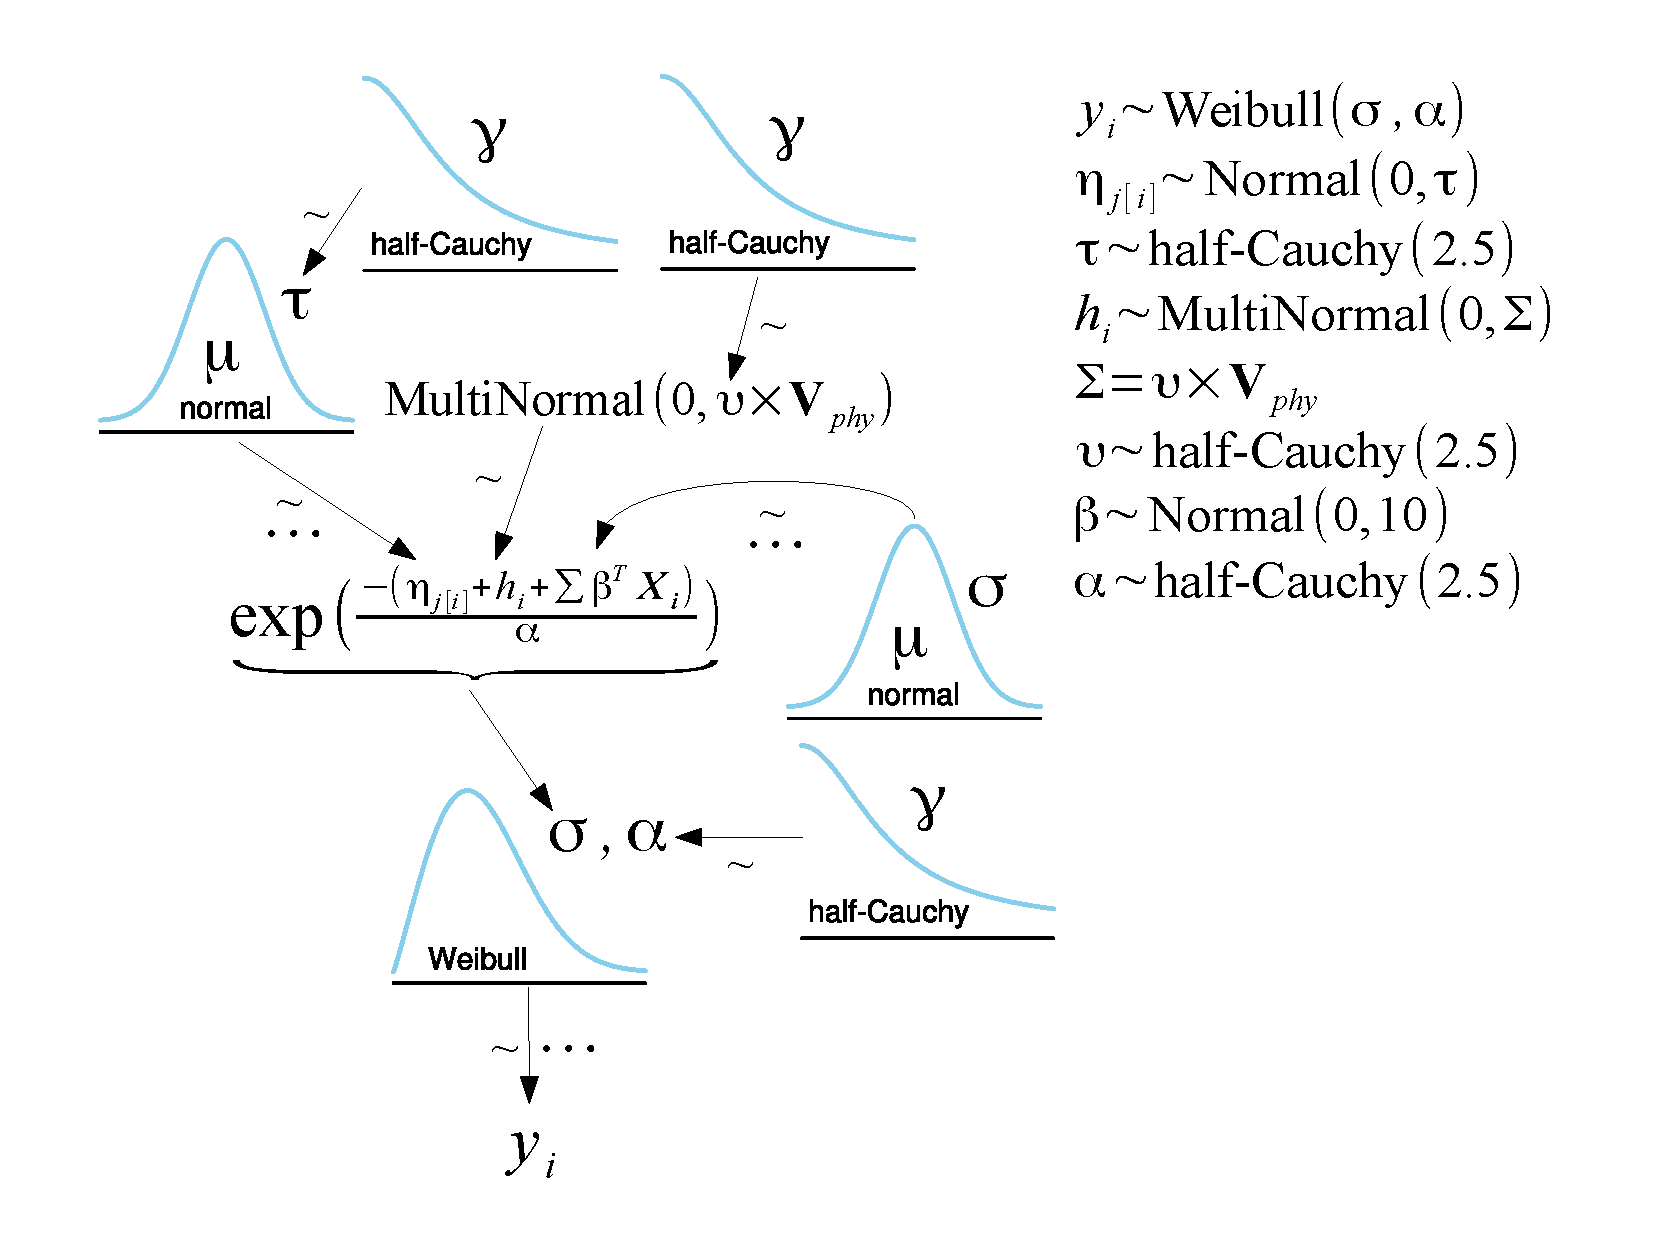
\includegraphics[height = 0.8\textheight, width = \textwidth,  keepaspectratio = true]{figure/mammal_survival_model}
  \end{center}
\end{frame}

\begin{frame}
  \frametitle{Censored observations}

  % visual/diagram slide?
  
  Right censored if not yet extinct

  ccdf (1 - cdf) at observed duration given model
  \begin{equation}
    \mathrm{Pr}[T > T_{i}] = \int_{T_{i}}^{\infty} \mathrm{Weibull}(T_{i} | \alpha, \sigma) dy = 1 - F(T_{i} | \alpha, \sigma)
    \label{eq:right_cen}
  \end{equation}
  

  Left censored if both extinct and only one stage

  cdf at obserged duration given model
  \begin{equation}
    \mathrm{Pr}[T < T_{i}] = \int_{-\infty}^{T_{i}} \mathrm{Weibull}(T_{i} | \alpha, \sigma) dy = F(T_{i} | \alpha, \sigma)
    \label{eq:left_cen}
  \end{equation}

\end{frame}

\begin{frame}
  \frametitle{Posterior predictive checks: S(t)}
  \begin{center}
    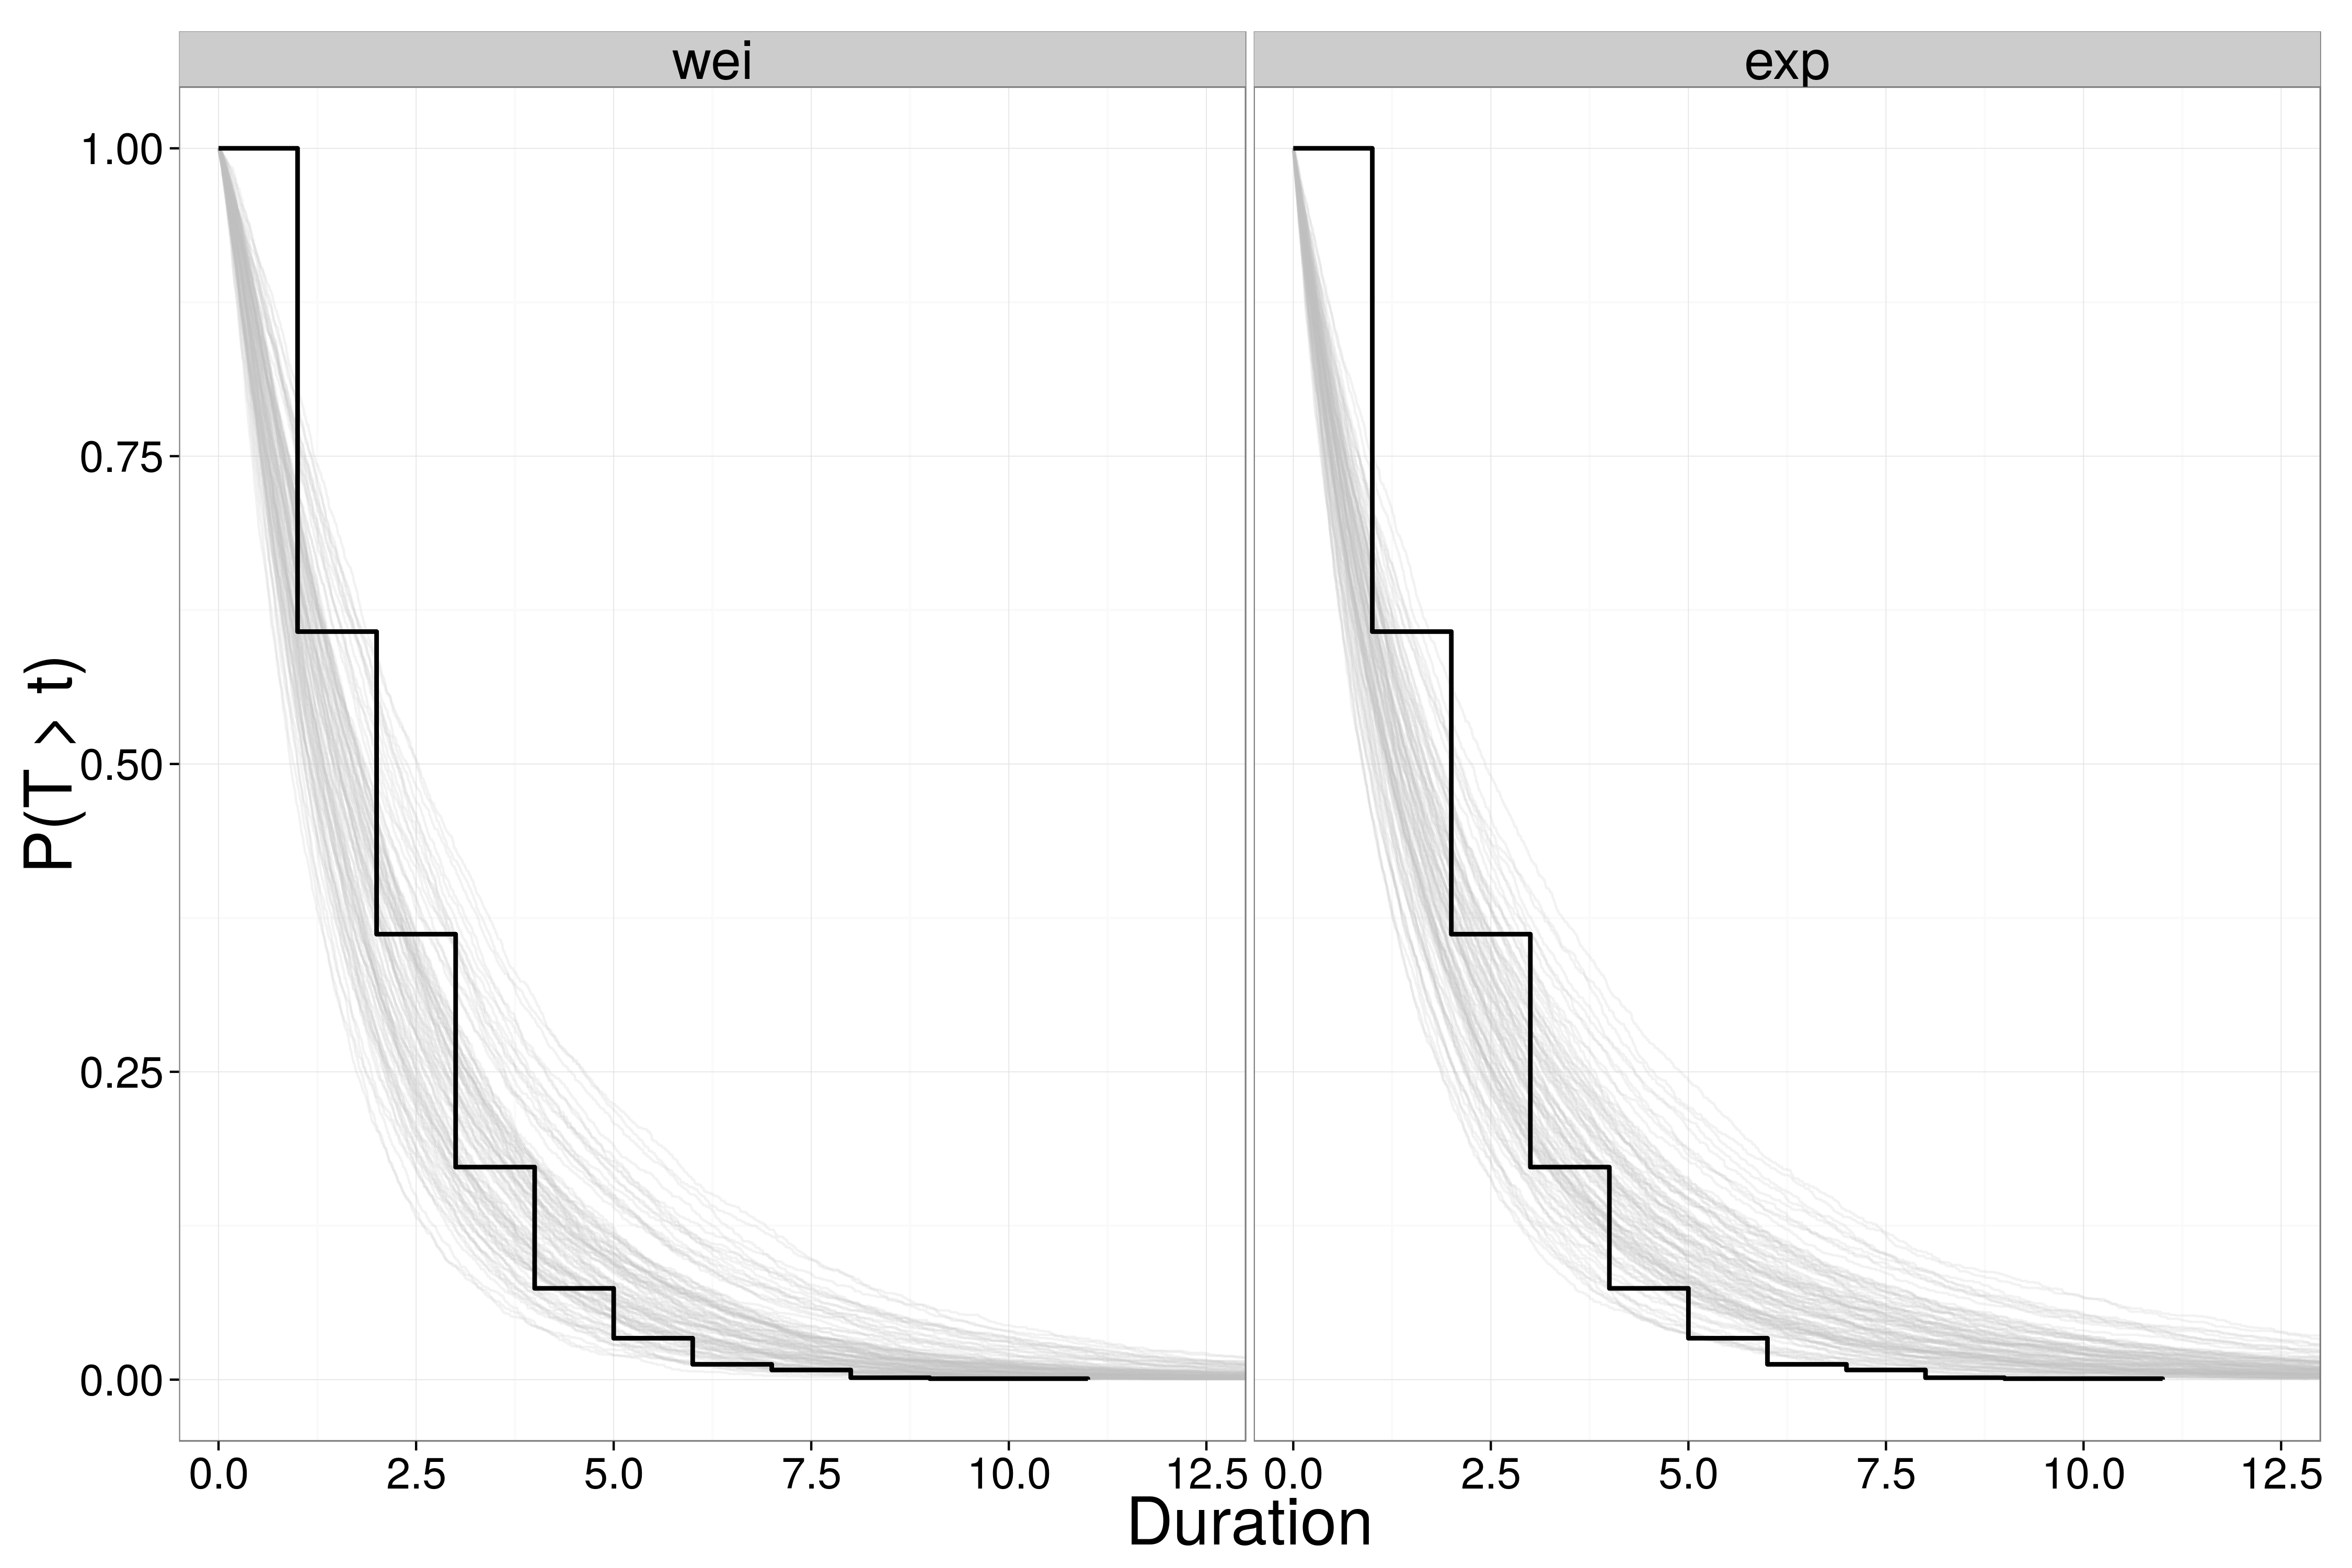
\includegraphics[height = 0.8\textheight, width = \textwidth,  keepaspectratio = true]{figure/survival_function}
  \end{center}
\end{frame}

\begin{frame}
  \frametitle{Posterior predictive checks: stnd. residuals}
  \begin{center}
    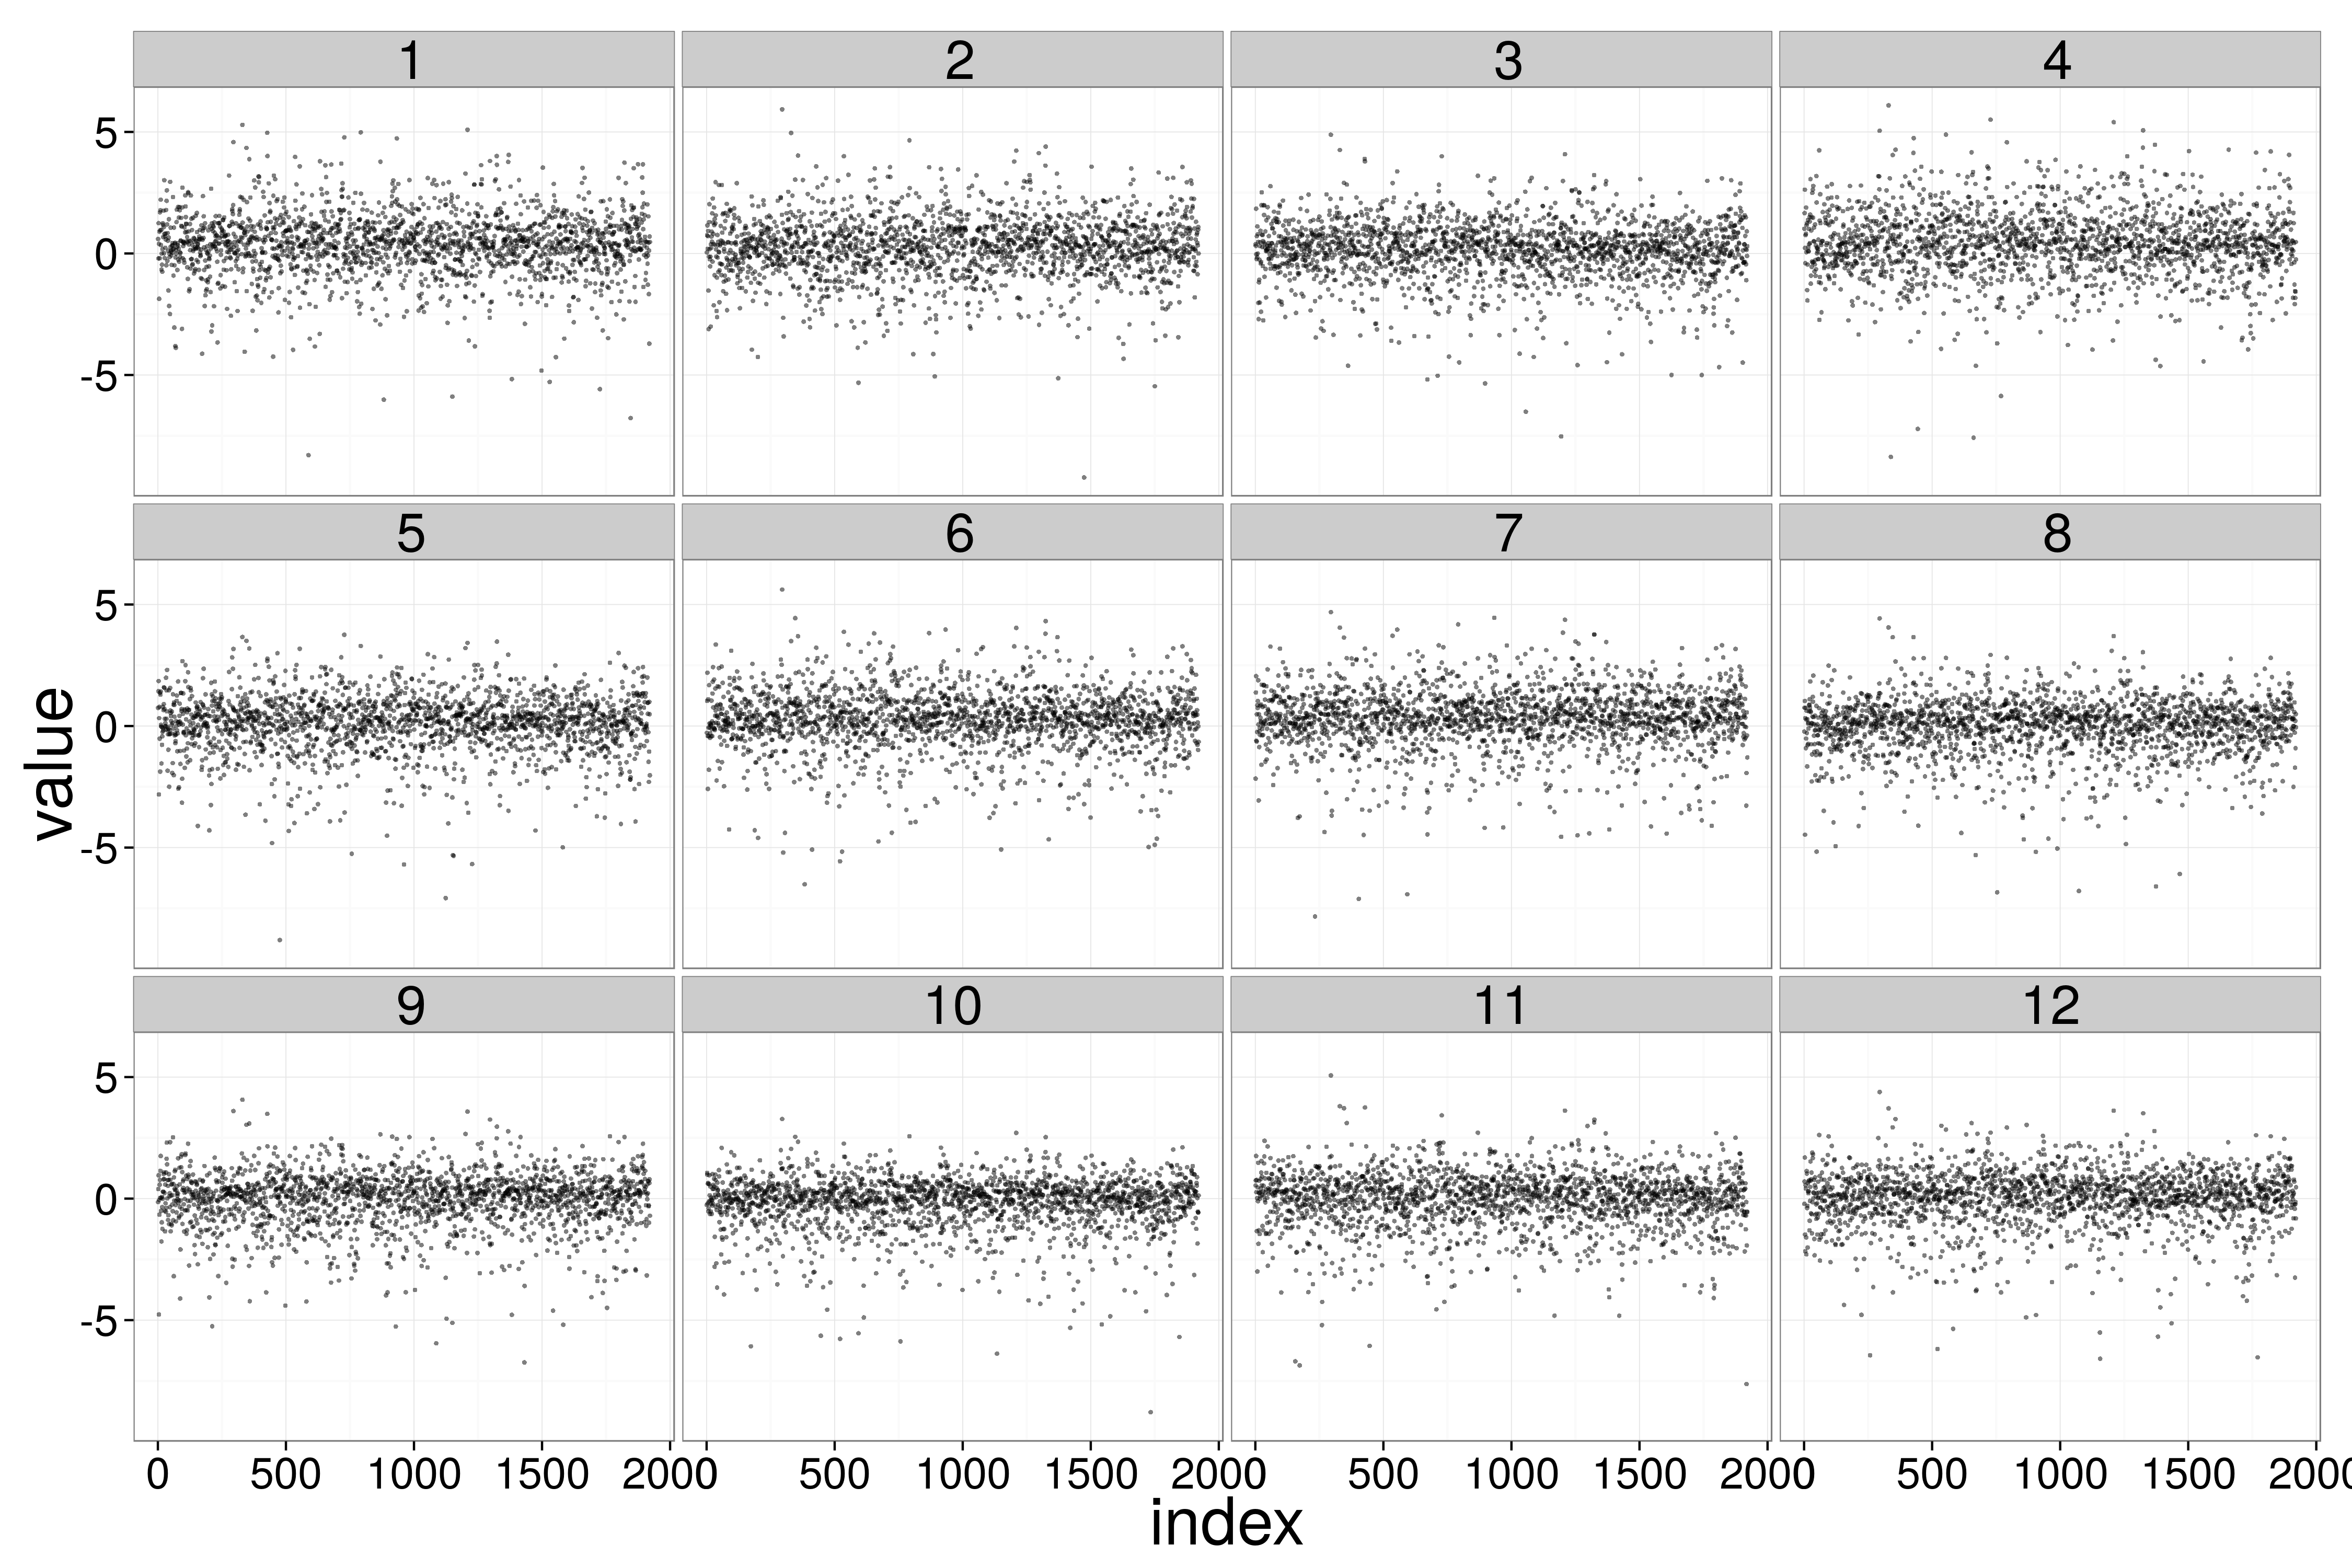
\includegraphics[height = 0.8\textheight, width = \textwidth,  keepaspectratio = true]{figure/residual_plot}
  \end{center}
\end{frame}

\begin{frame}
  \frametitle{Posterior predictive checks: residuals and mean}
  \begin{columns}
    \begin{column}{0.5\textwidth}
      \begin{center}
        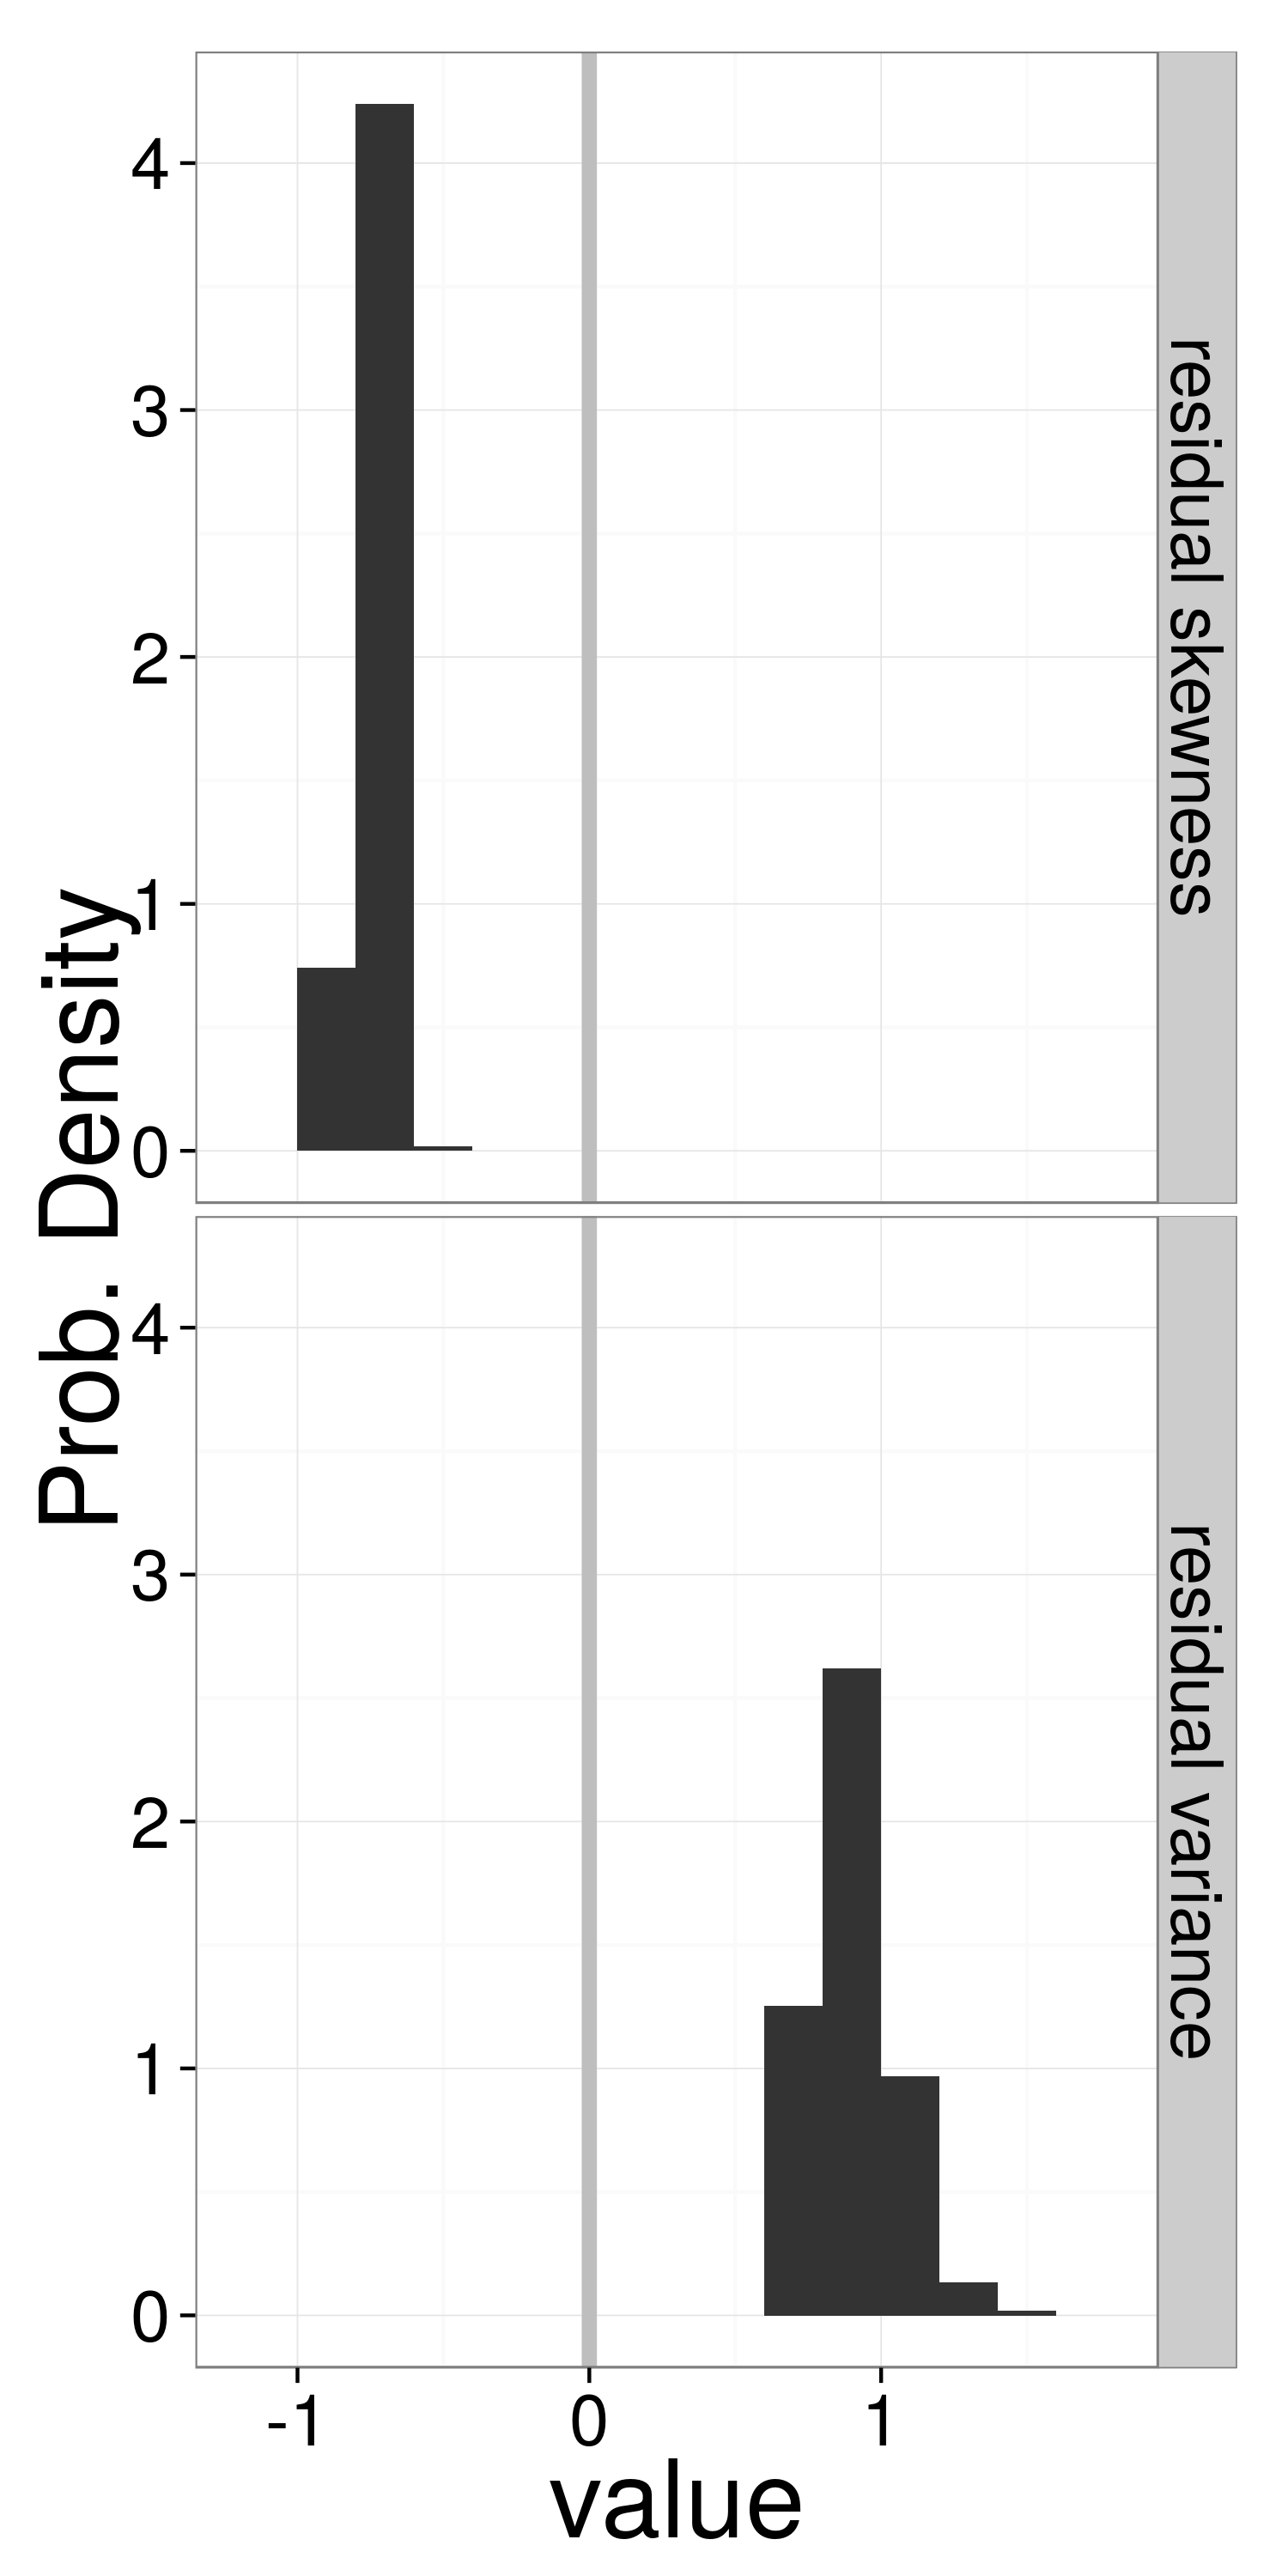
\includegraphics[height = 0.8\textheight, width = \textwidth,  keepaspectratio = true]{figure/res_sum_plot}
      \end{center}
    \end{column}
    \begin{column}{0.5\textwidth}
      \begin{center}
        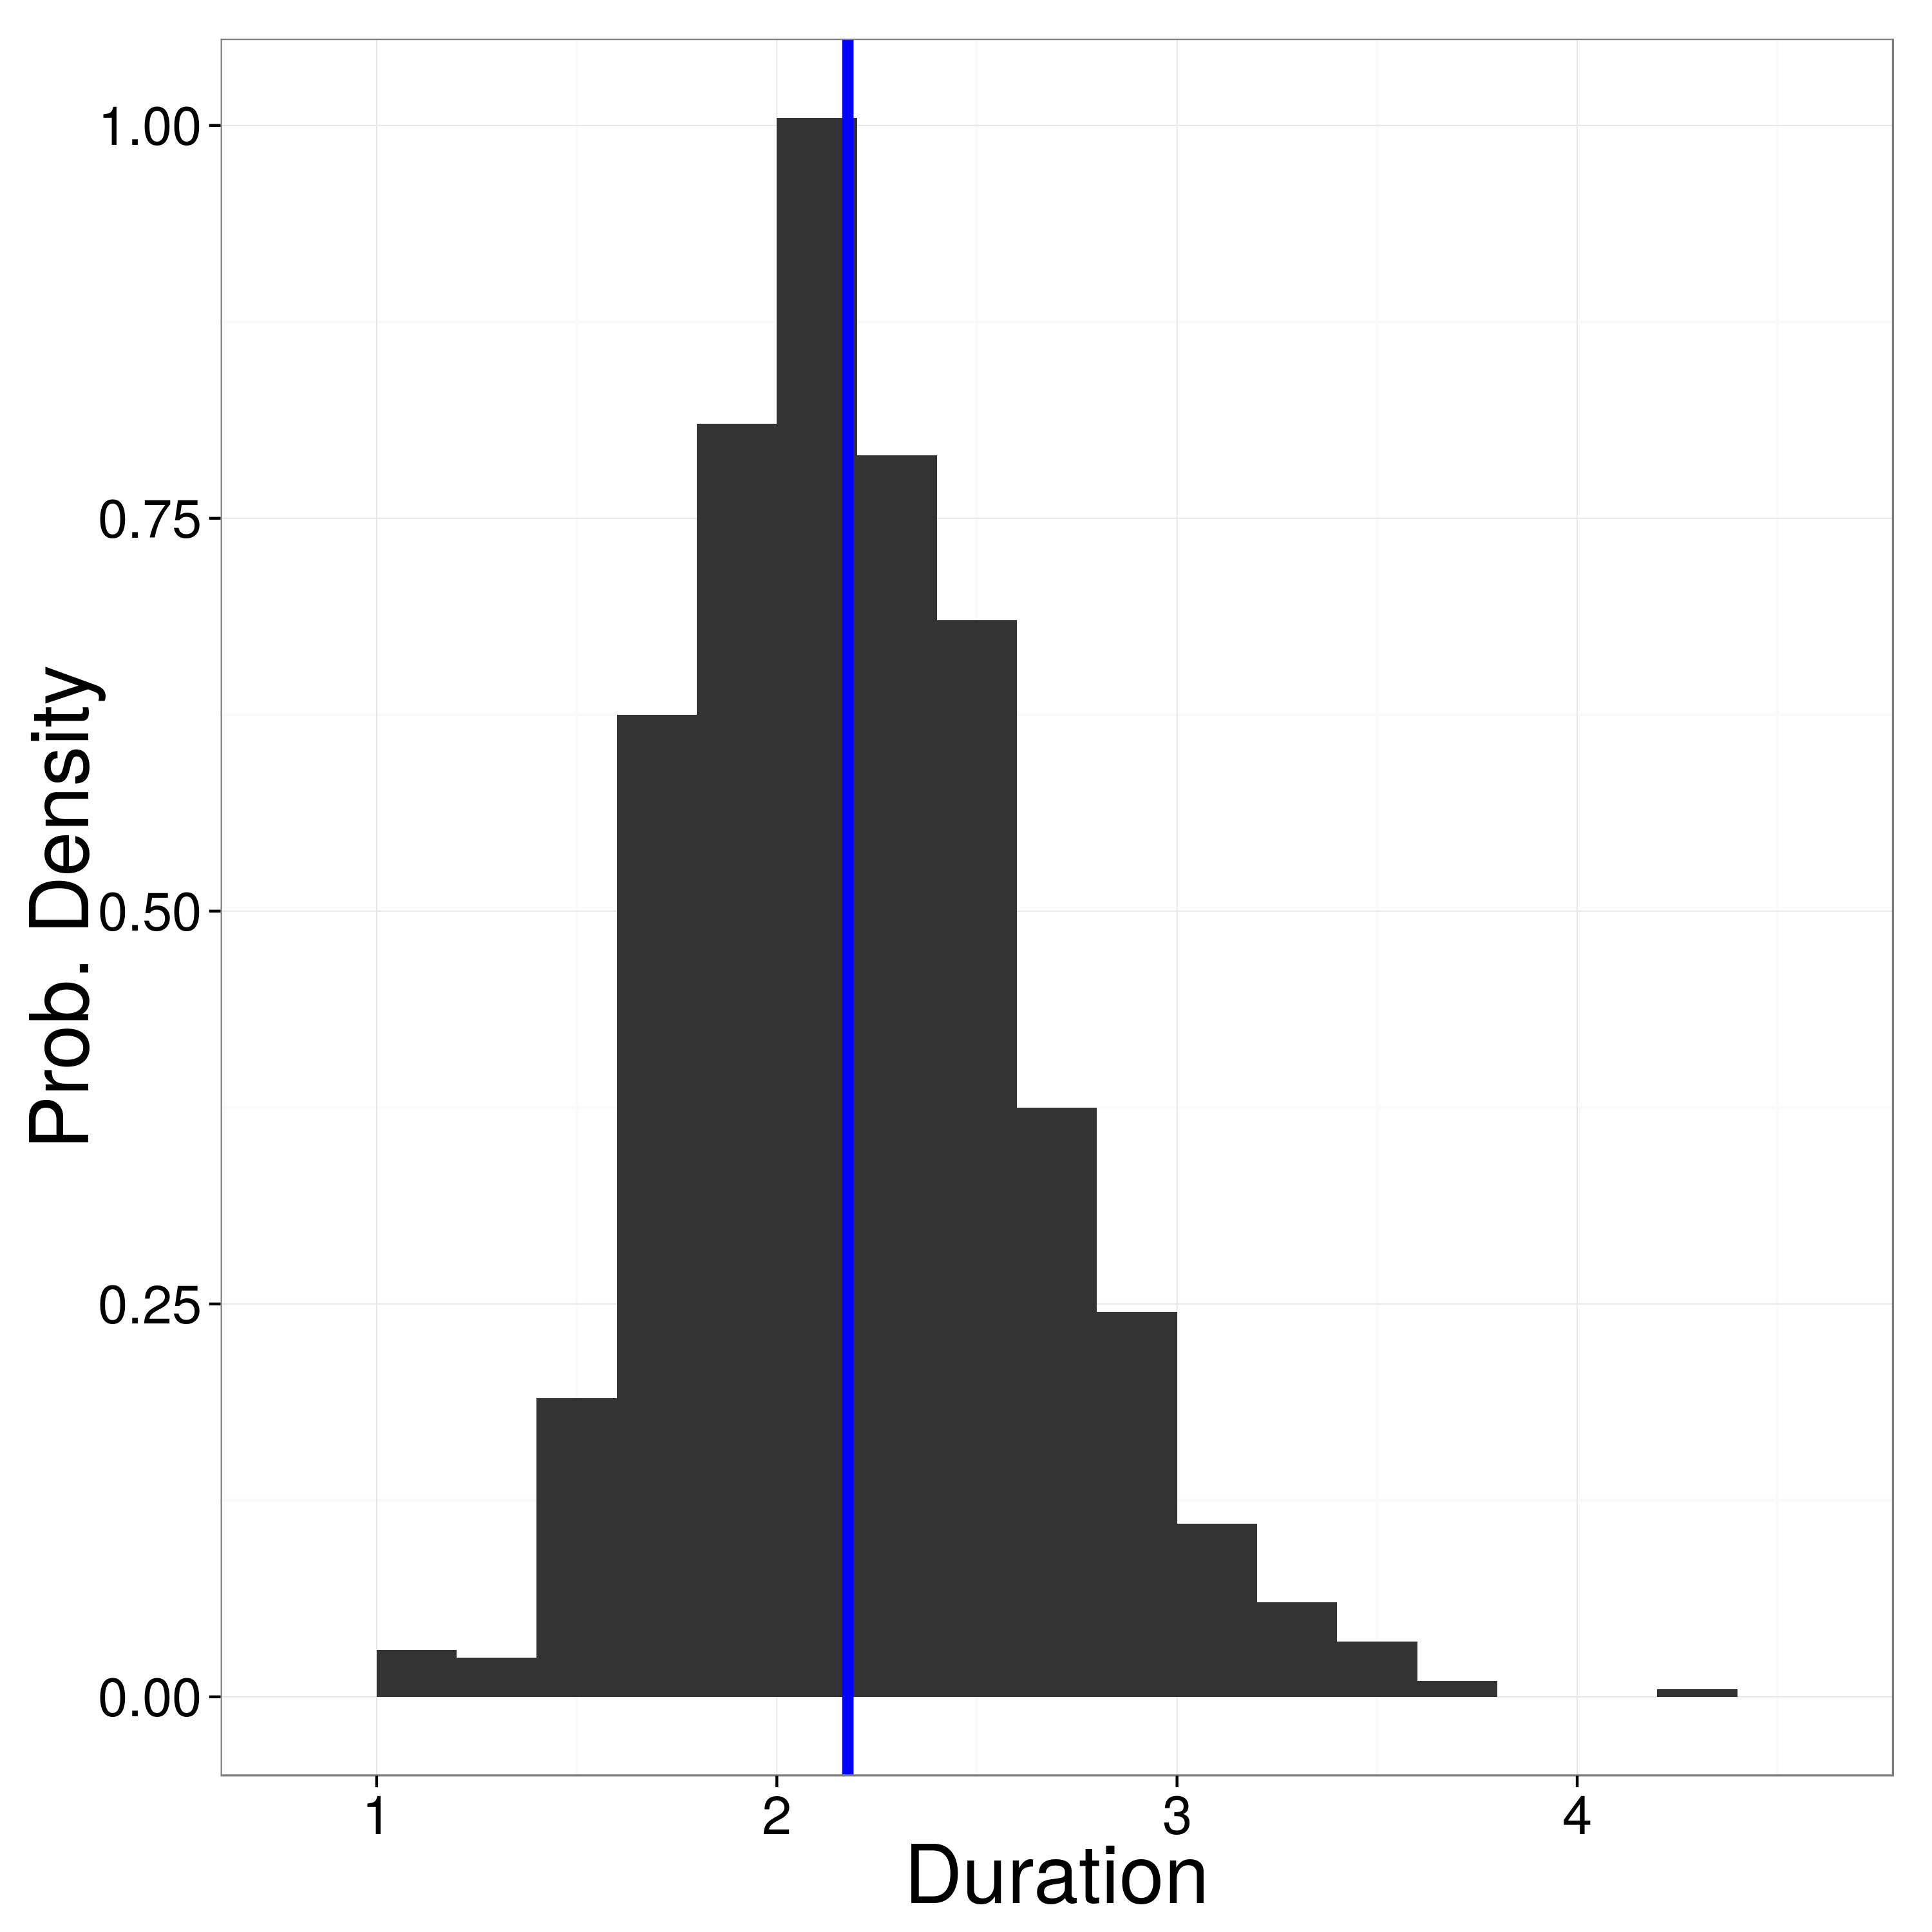
\includegraphics[height = 0.8\textheight, width = \textwidth,  keepaspectratio = true]{figure/mean_ppc}
      \end{center}
    \end{column}
  \end{columns}
\end{frame}

\begin{frame}
  \frametitle{Pairwise differences of \(\beta\), dietary category}
  \begin{center}
    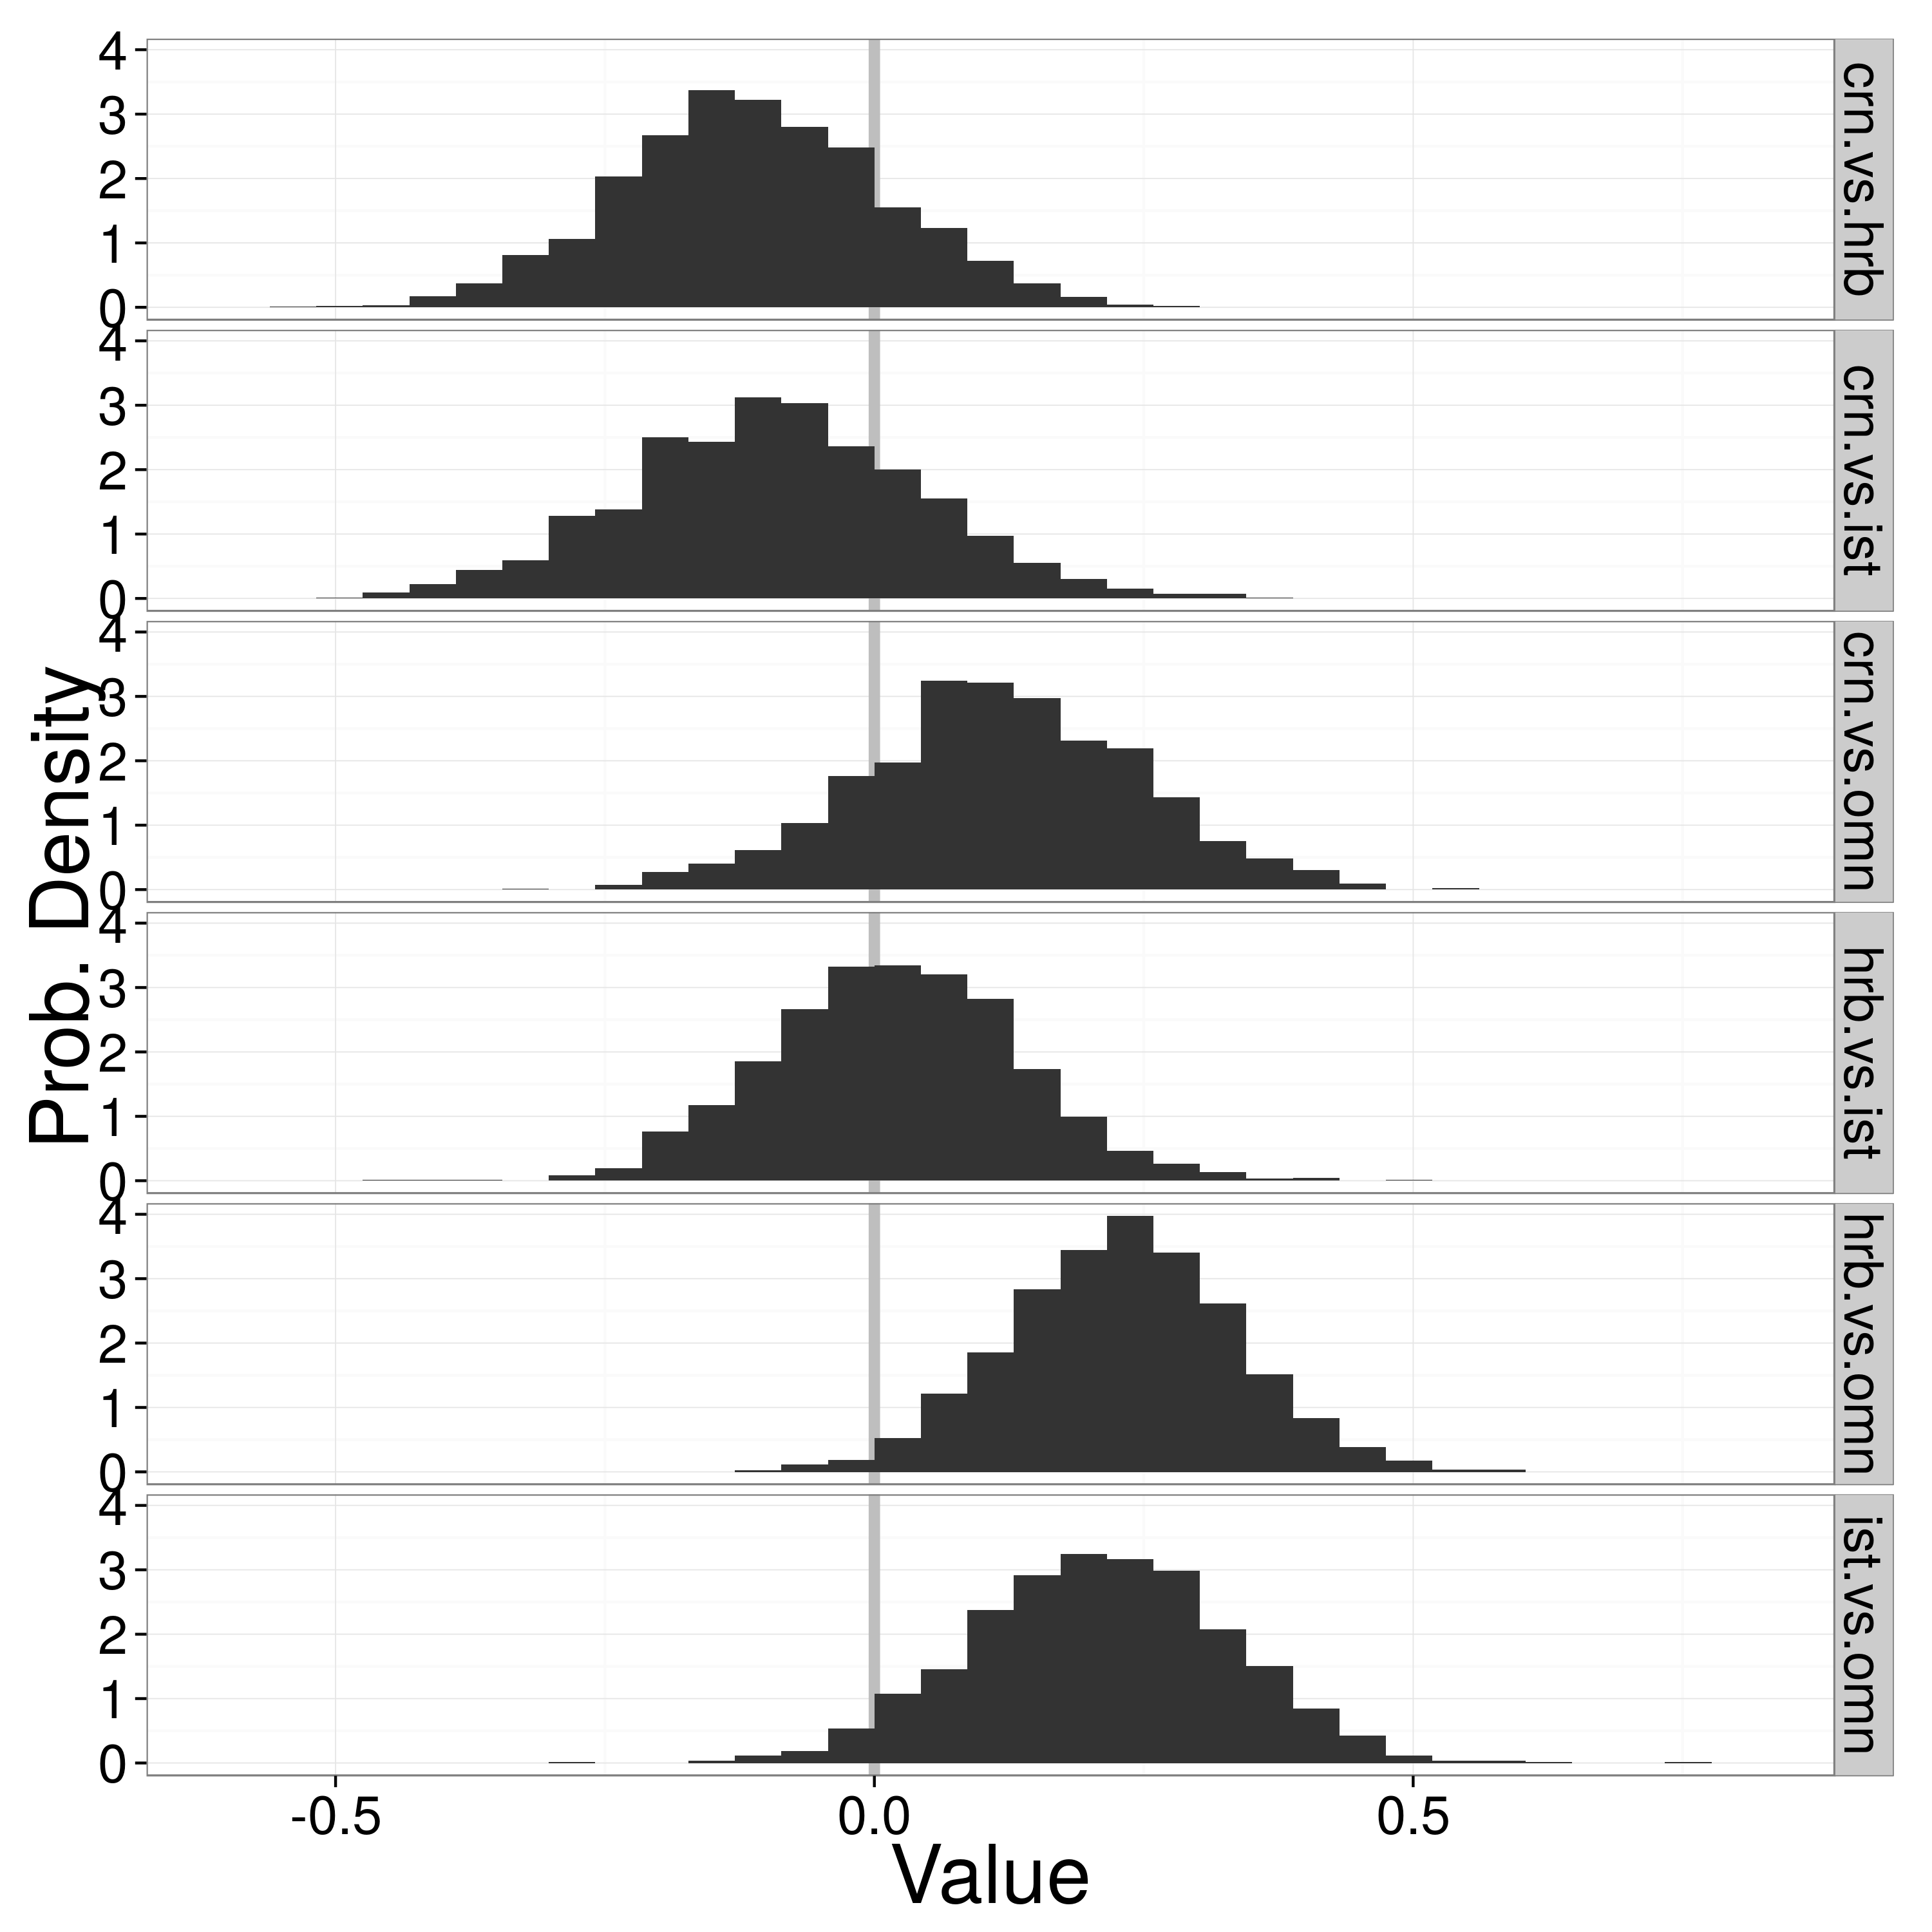
\includegraphics[height = 0.8\textheight, width = \textwidth,  keepaspectratio = true]{figure/diet_diff_est}
  \end{center}
\end{frame}

\begin{frame}
  \frametitle{Pairwise differences of \(\beta\), locomotor category}
  \begin{center}
    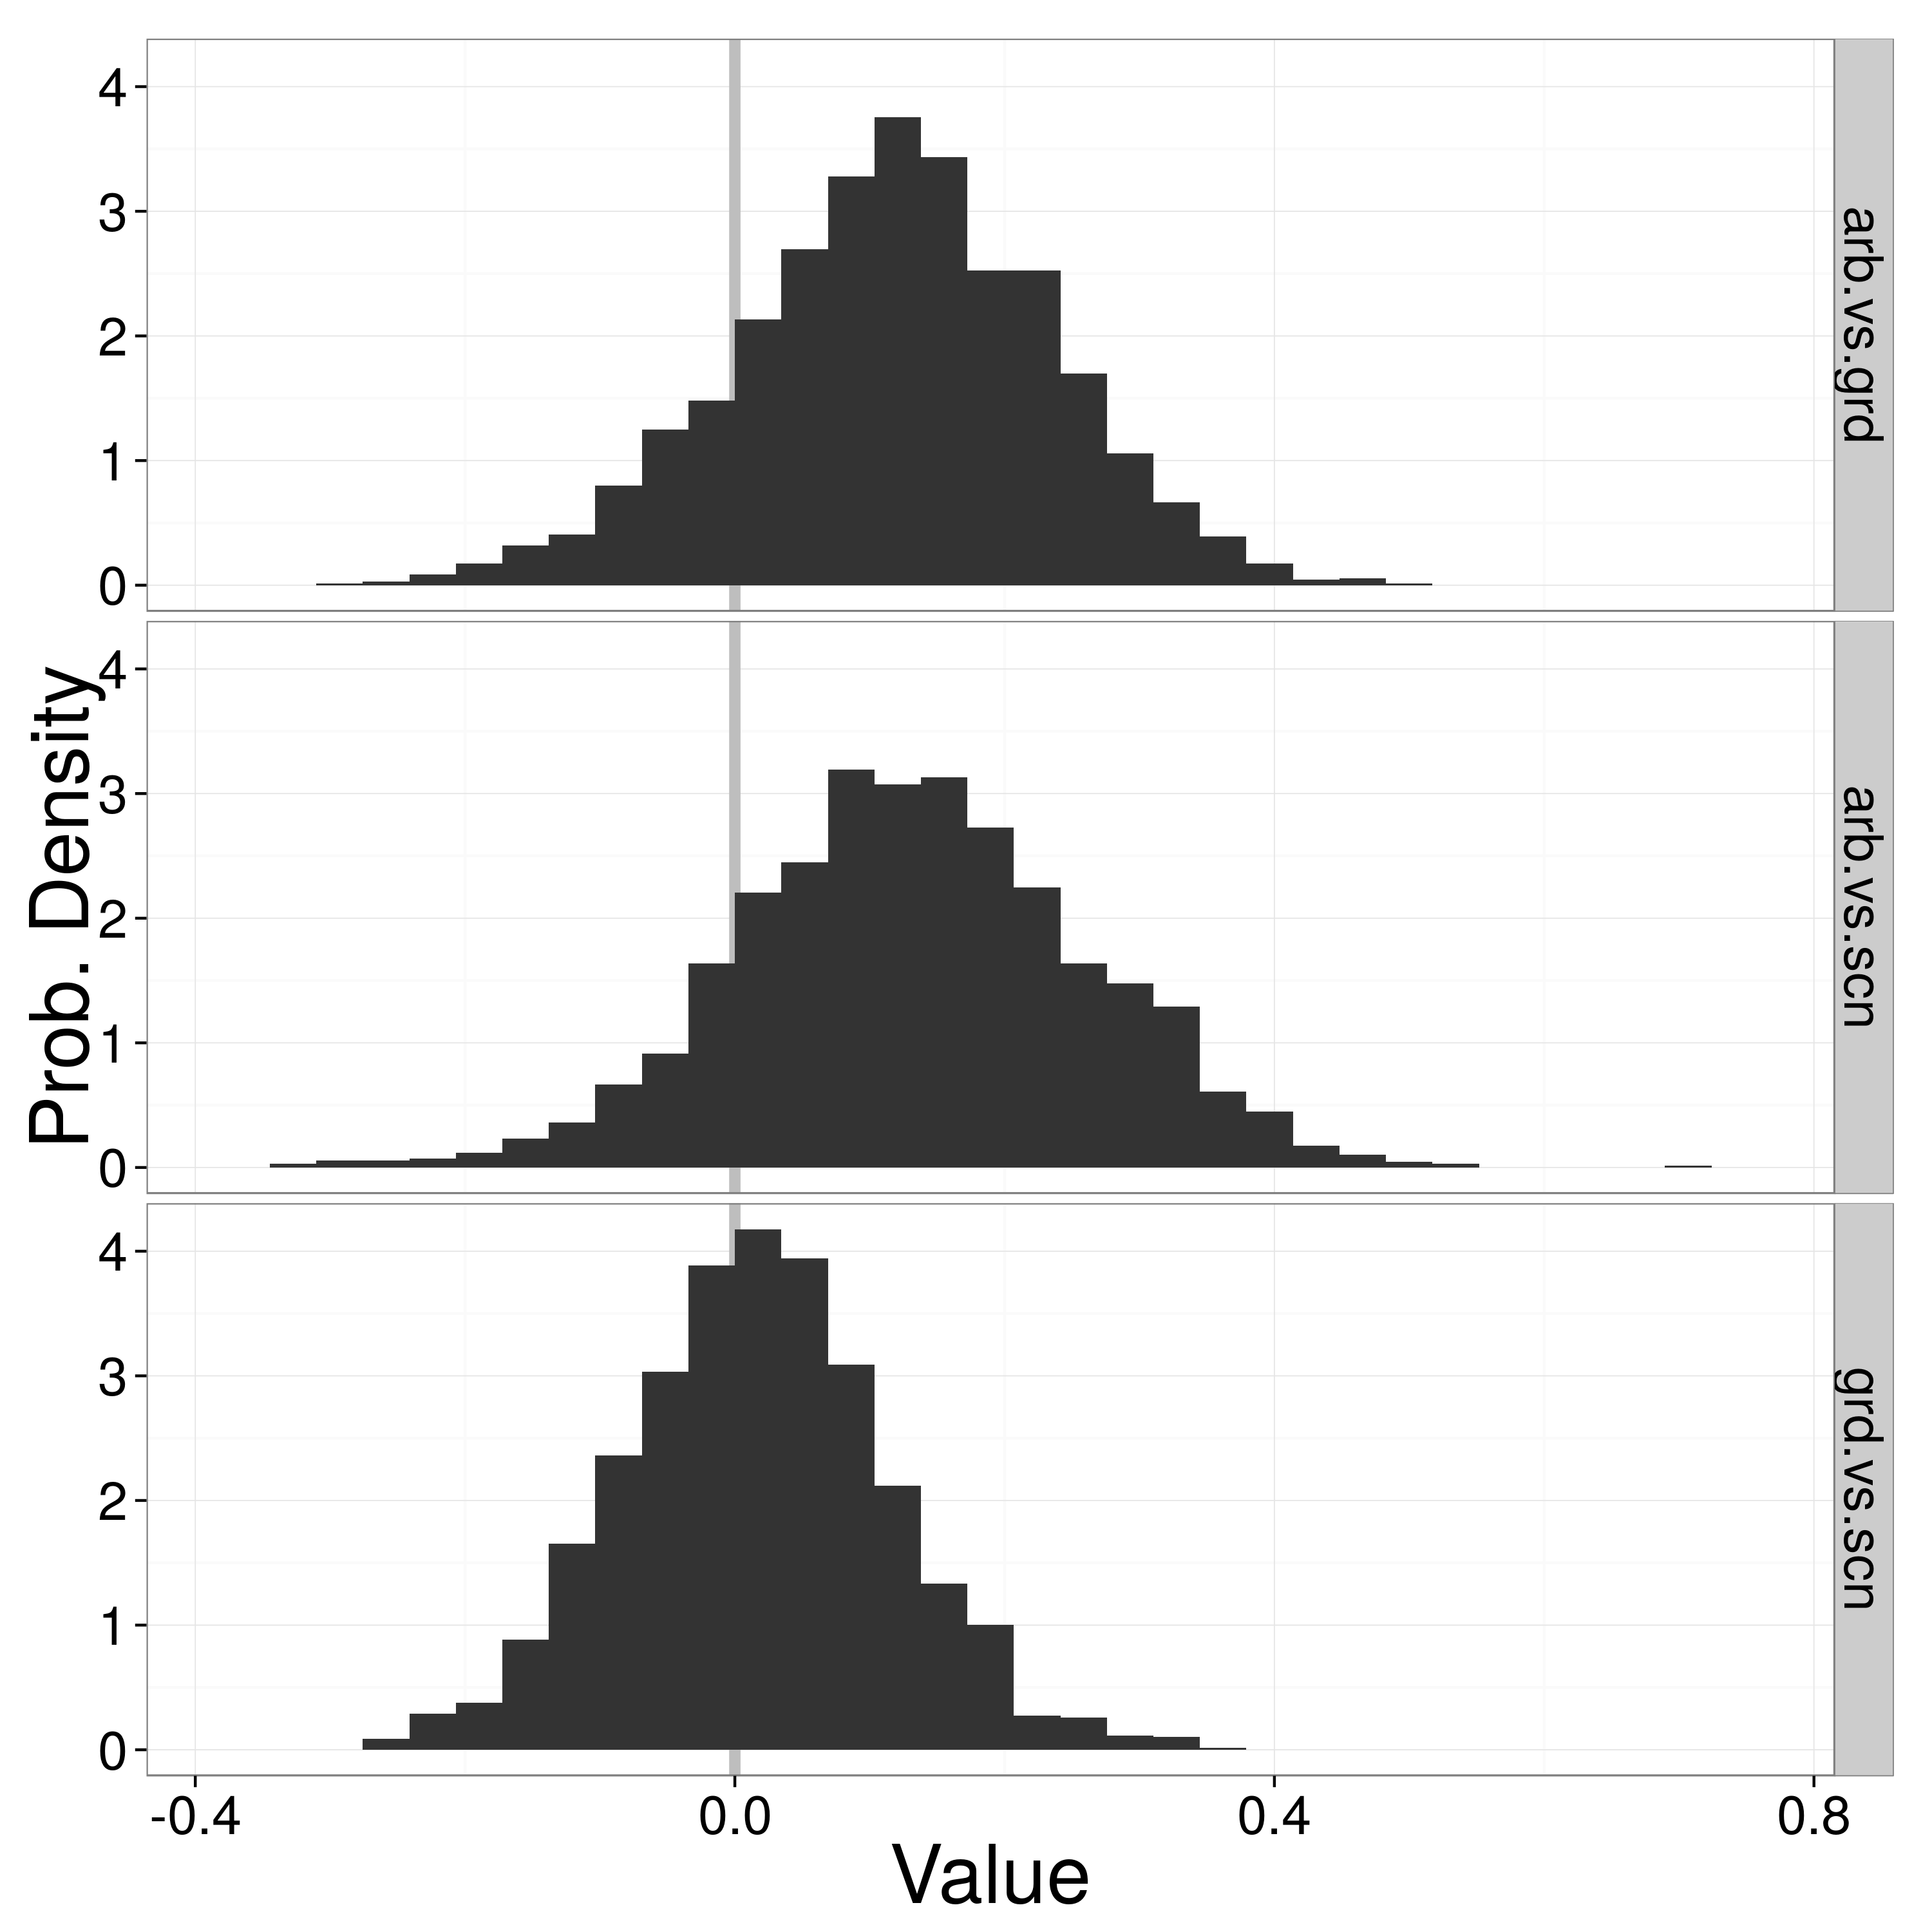
\includegraphics[height = 0.8\textheight, width = \textwidth,  keepaspectratio = true]{figure/loco_diff_est}
  \end{center}
\end{frame}

\begin{frame}
  \frametitle{Other traits}
  \begin{center}
    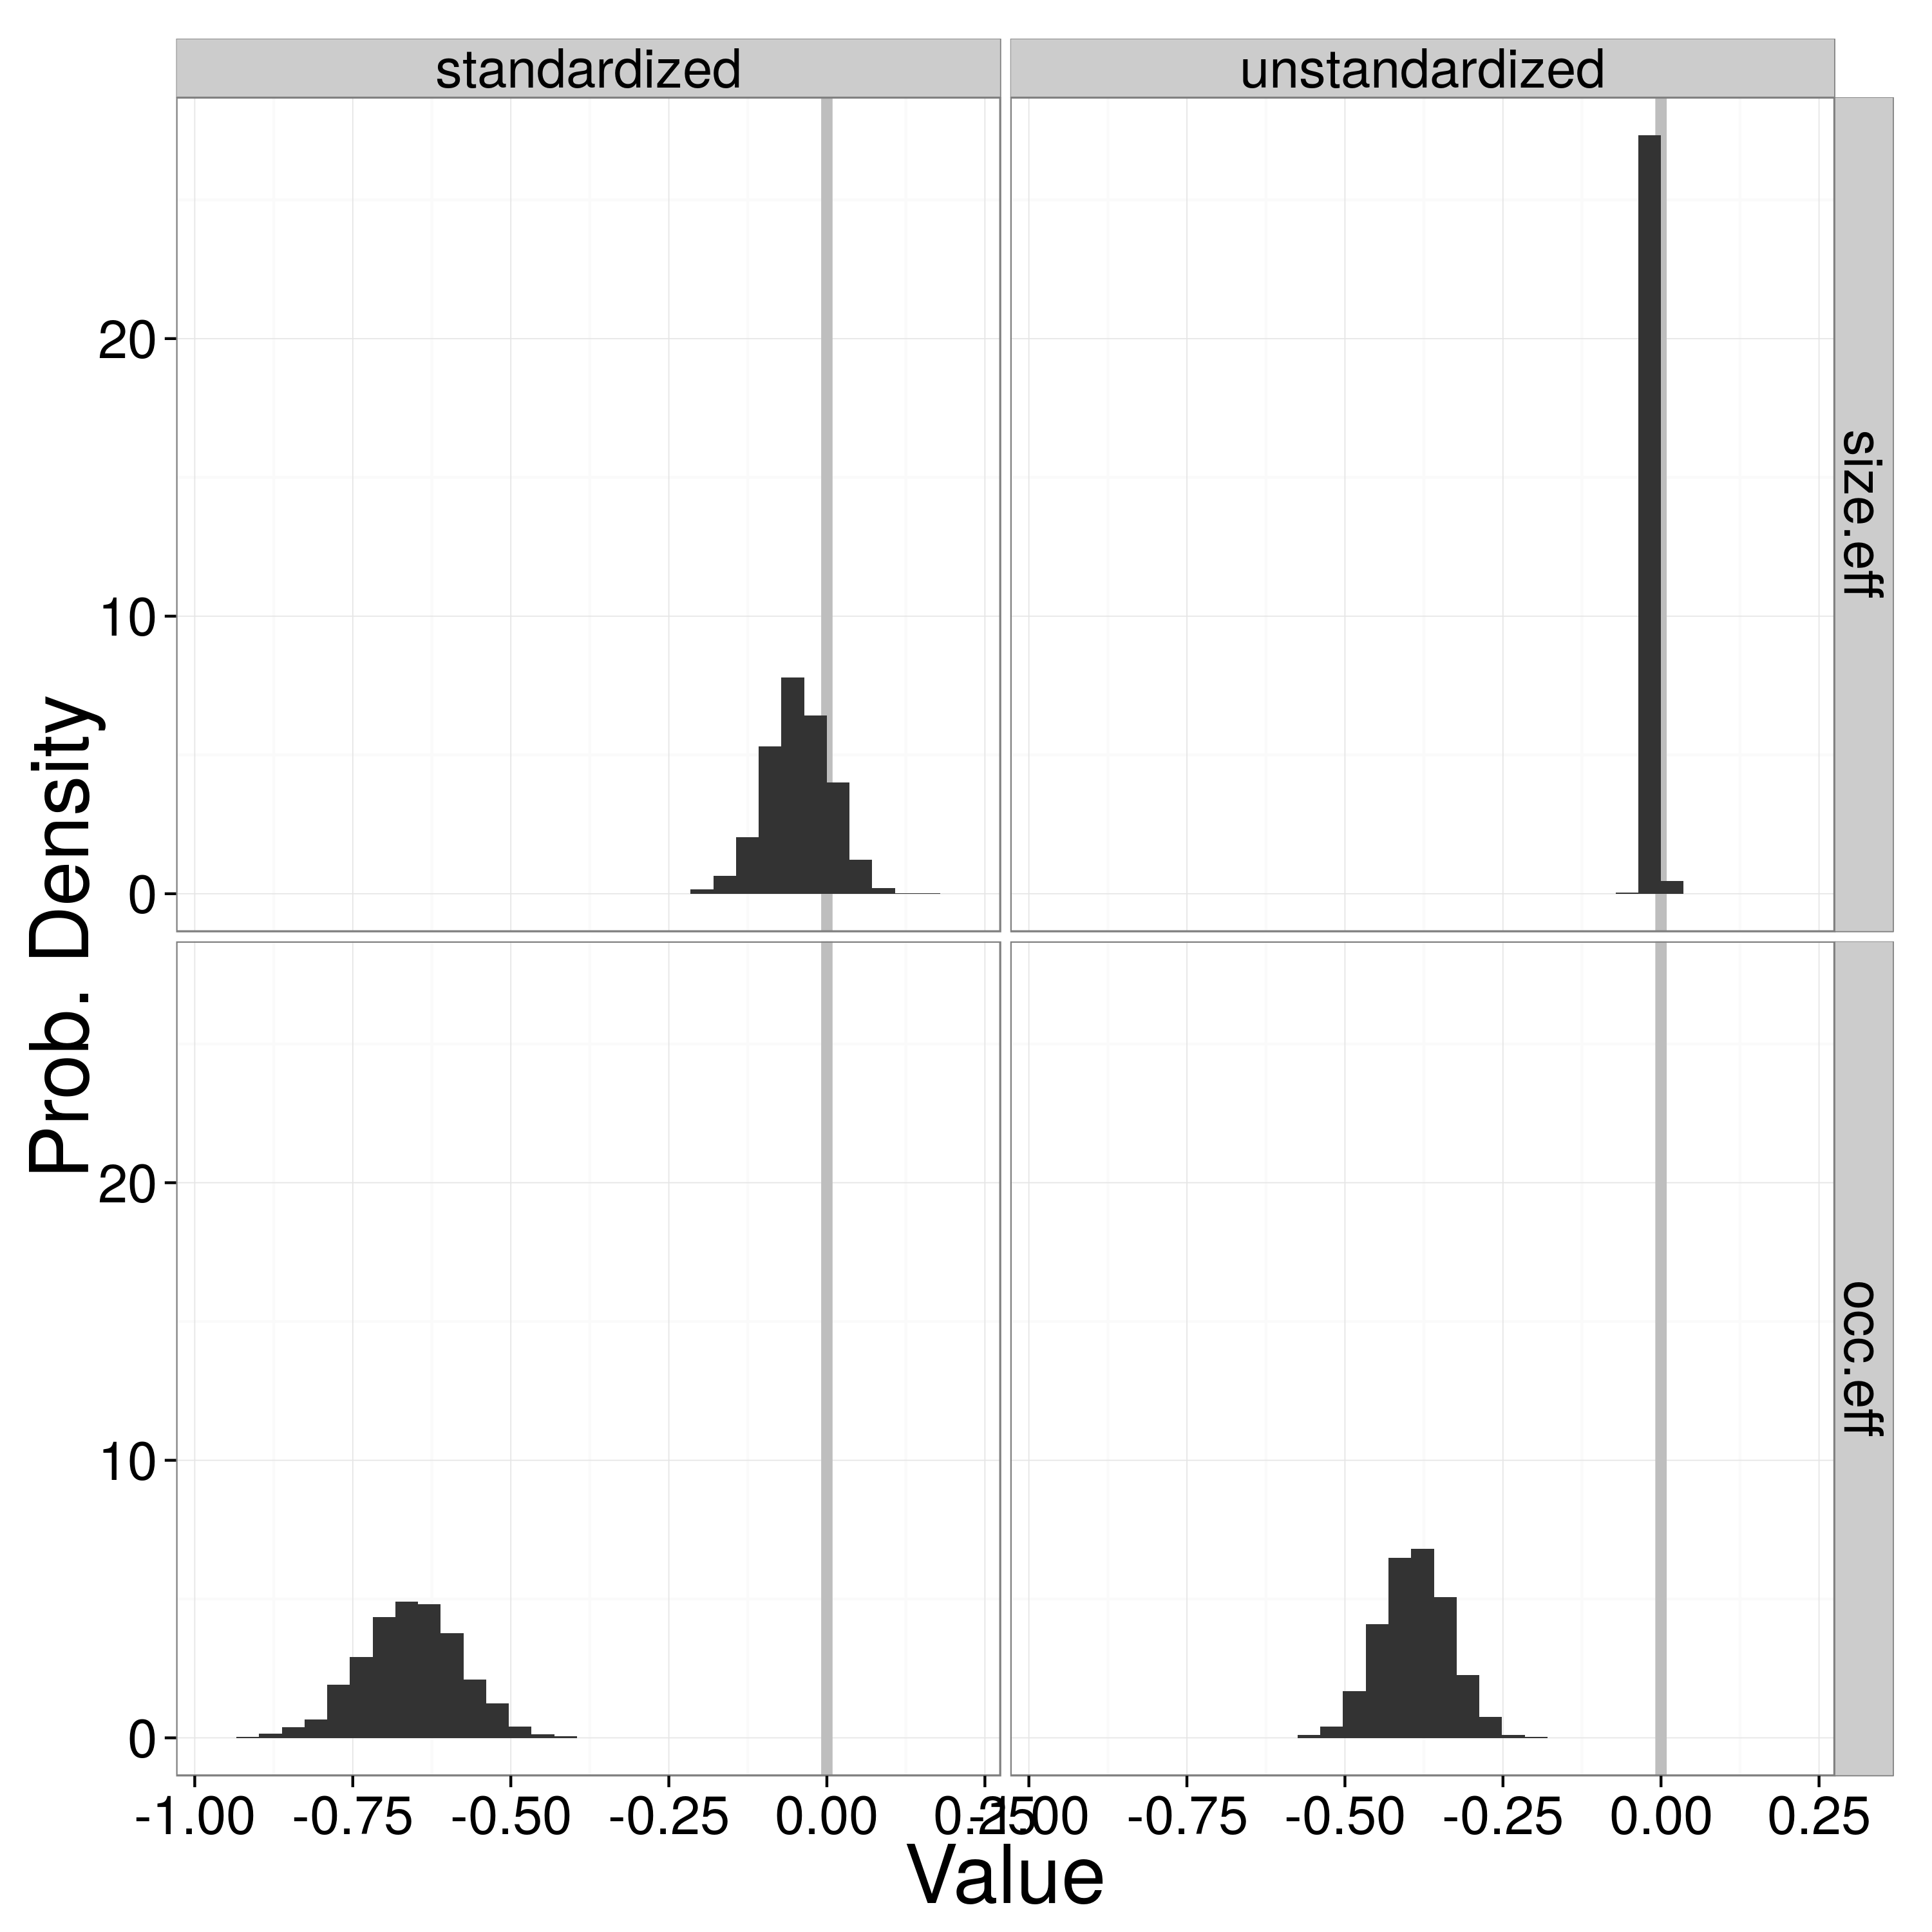
\includegraphics[height = 0.8\textheight, width = \textwidth,  keepaspectratio = true]{figure/other_est}
  \end{center}
\end{frame}

\begin{frame}
  \frametitle{Cohort effect}
  \begin{center}
    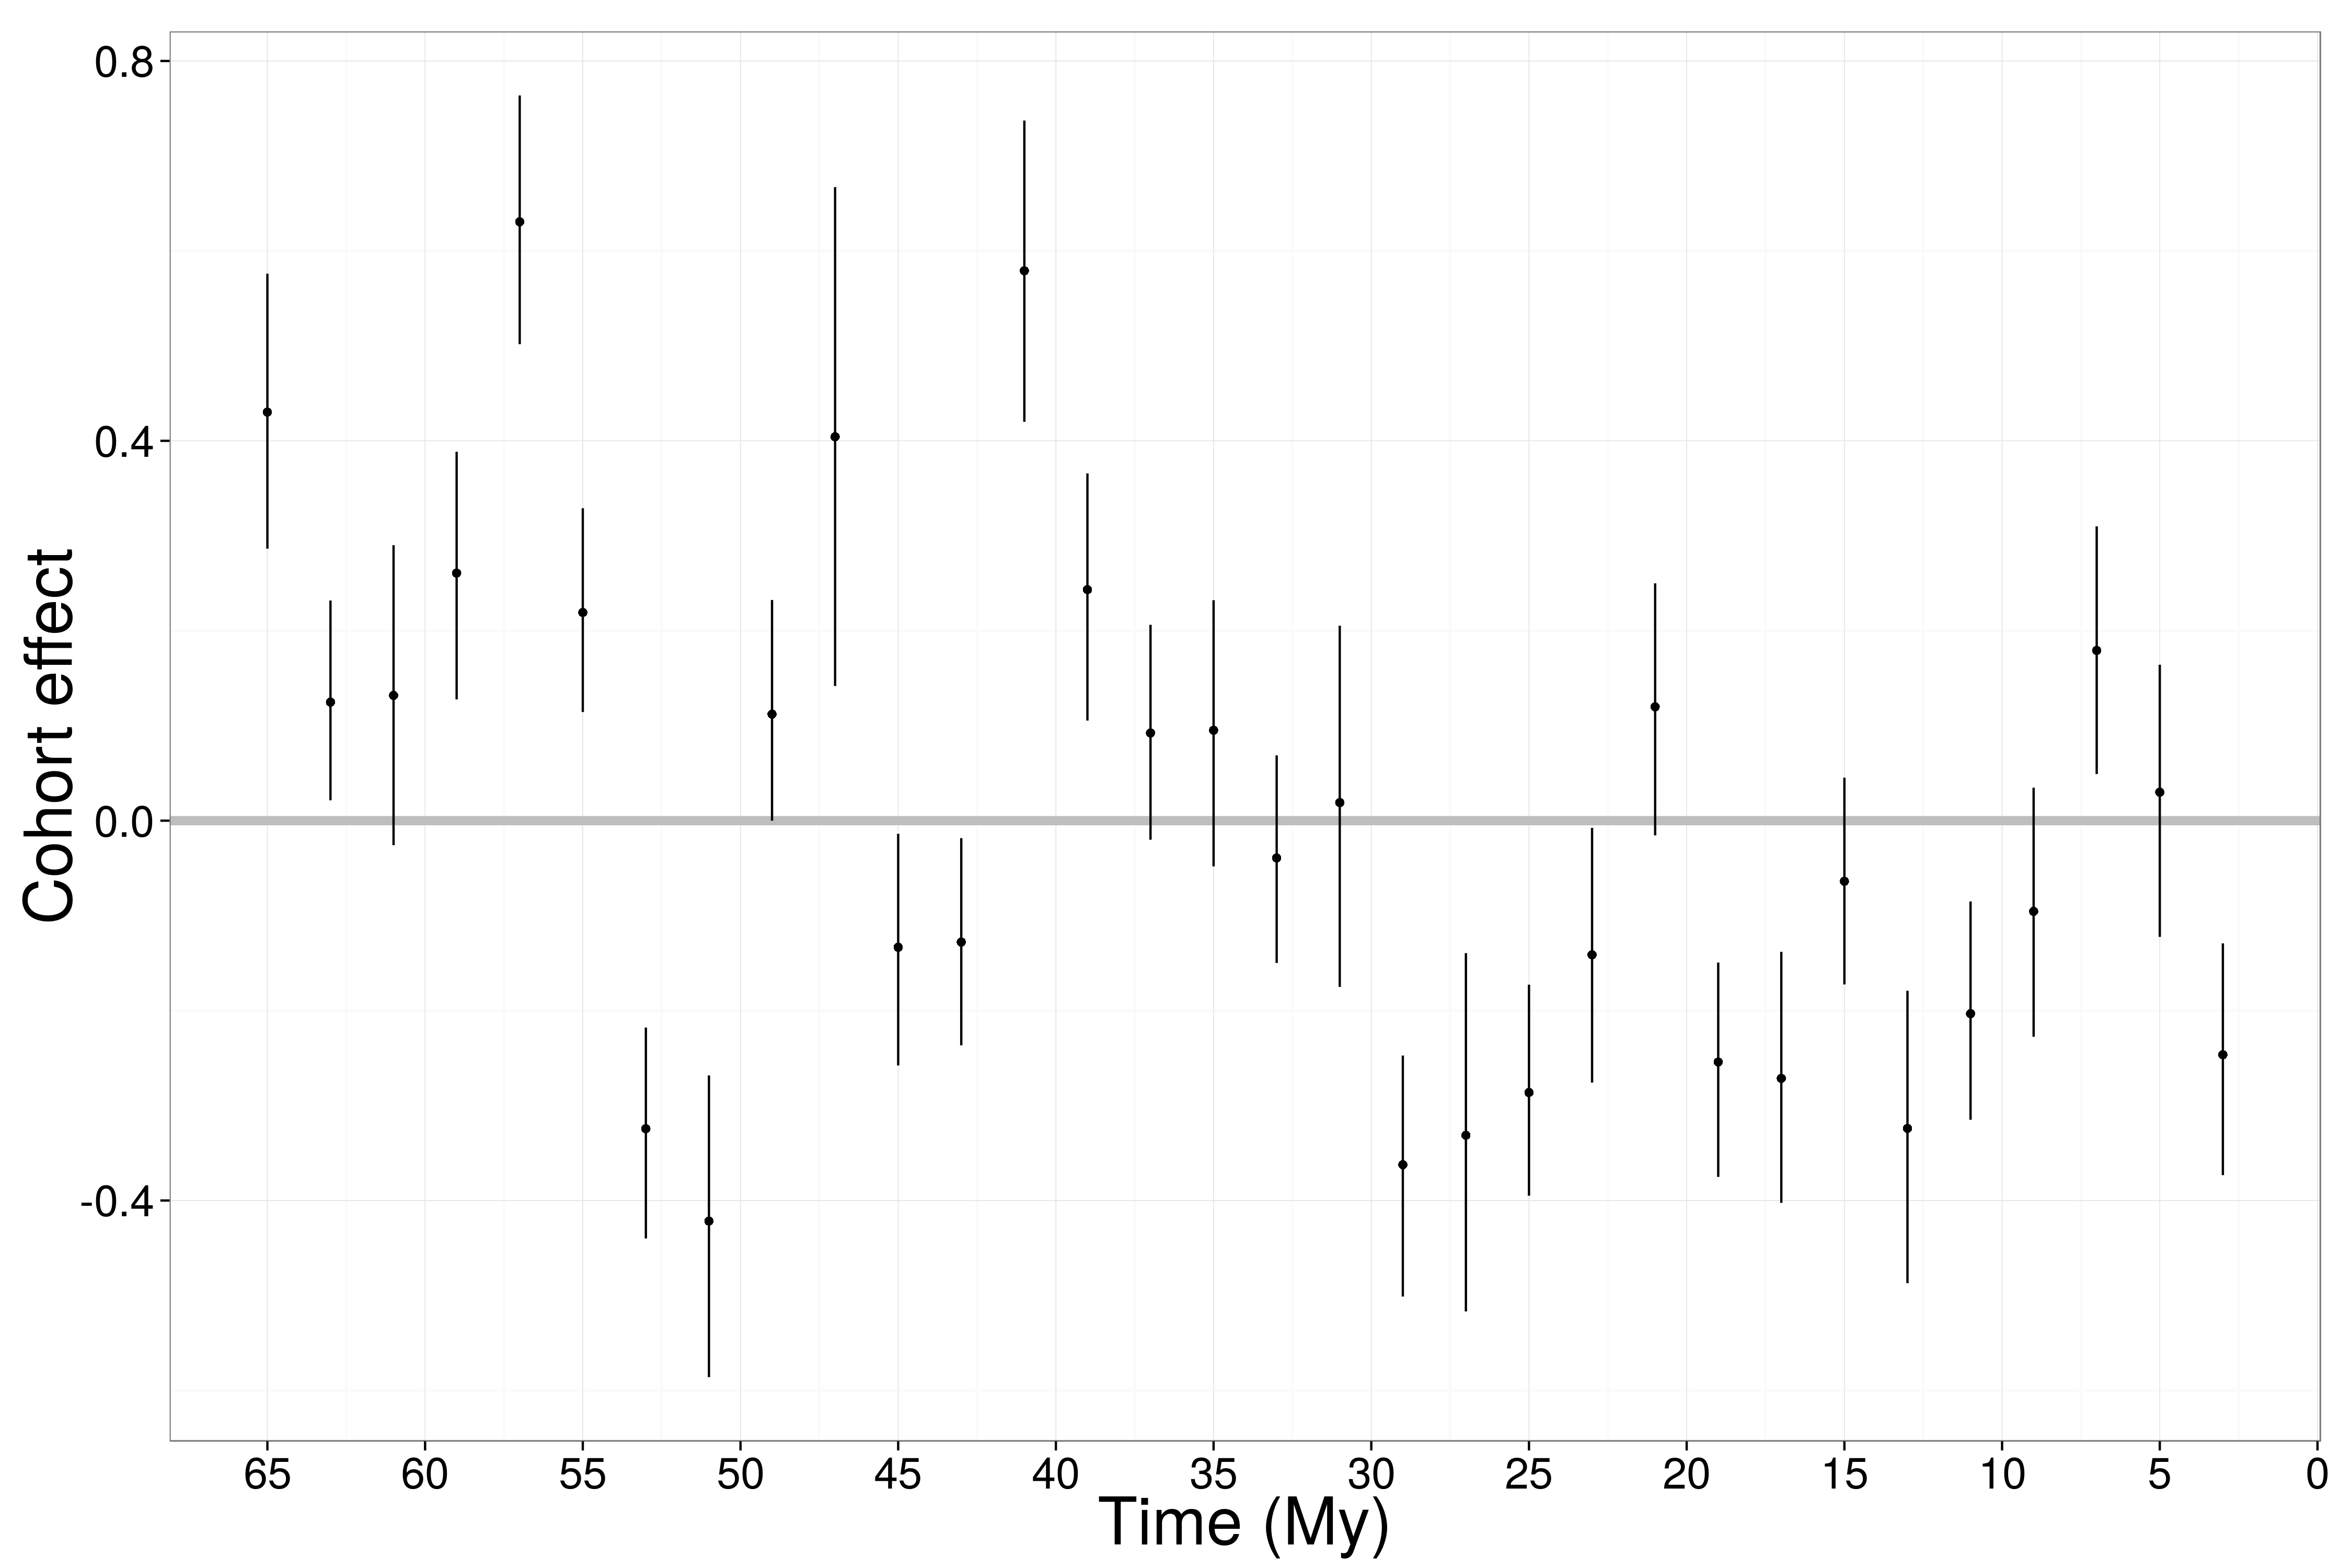
\includegraphics[height = 0.8\textheight, width = \textwidth,  keepaspectratio = true]{figure/cohort_est}
  \end{center}
\end{frame}

% something about the partial pooling, see Gelman and Hill 04

\begin{frame}
  \frametitle{Phylogenetic heritability \textit{sensu} Lynch '91}
\end{frame}

\begin{frame}
  \frametitle{Hazard curvature}
  \begin{center}
    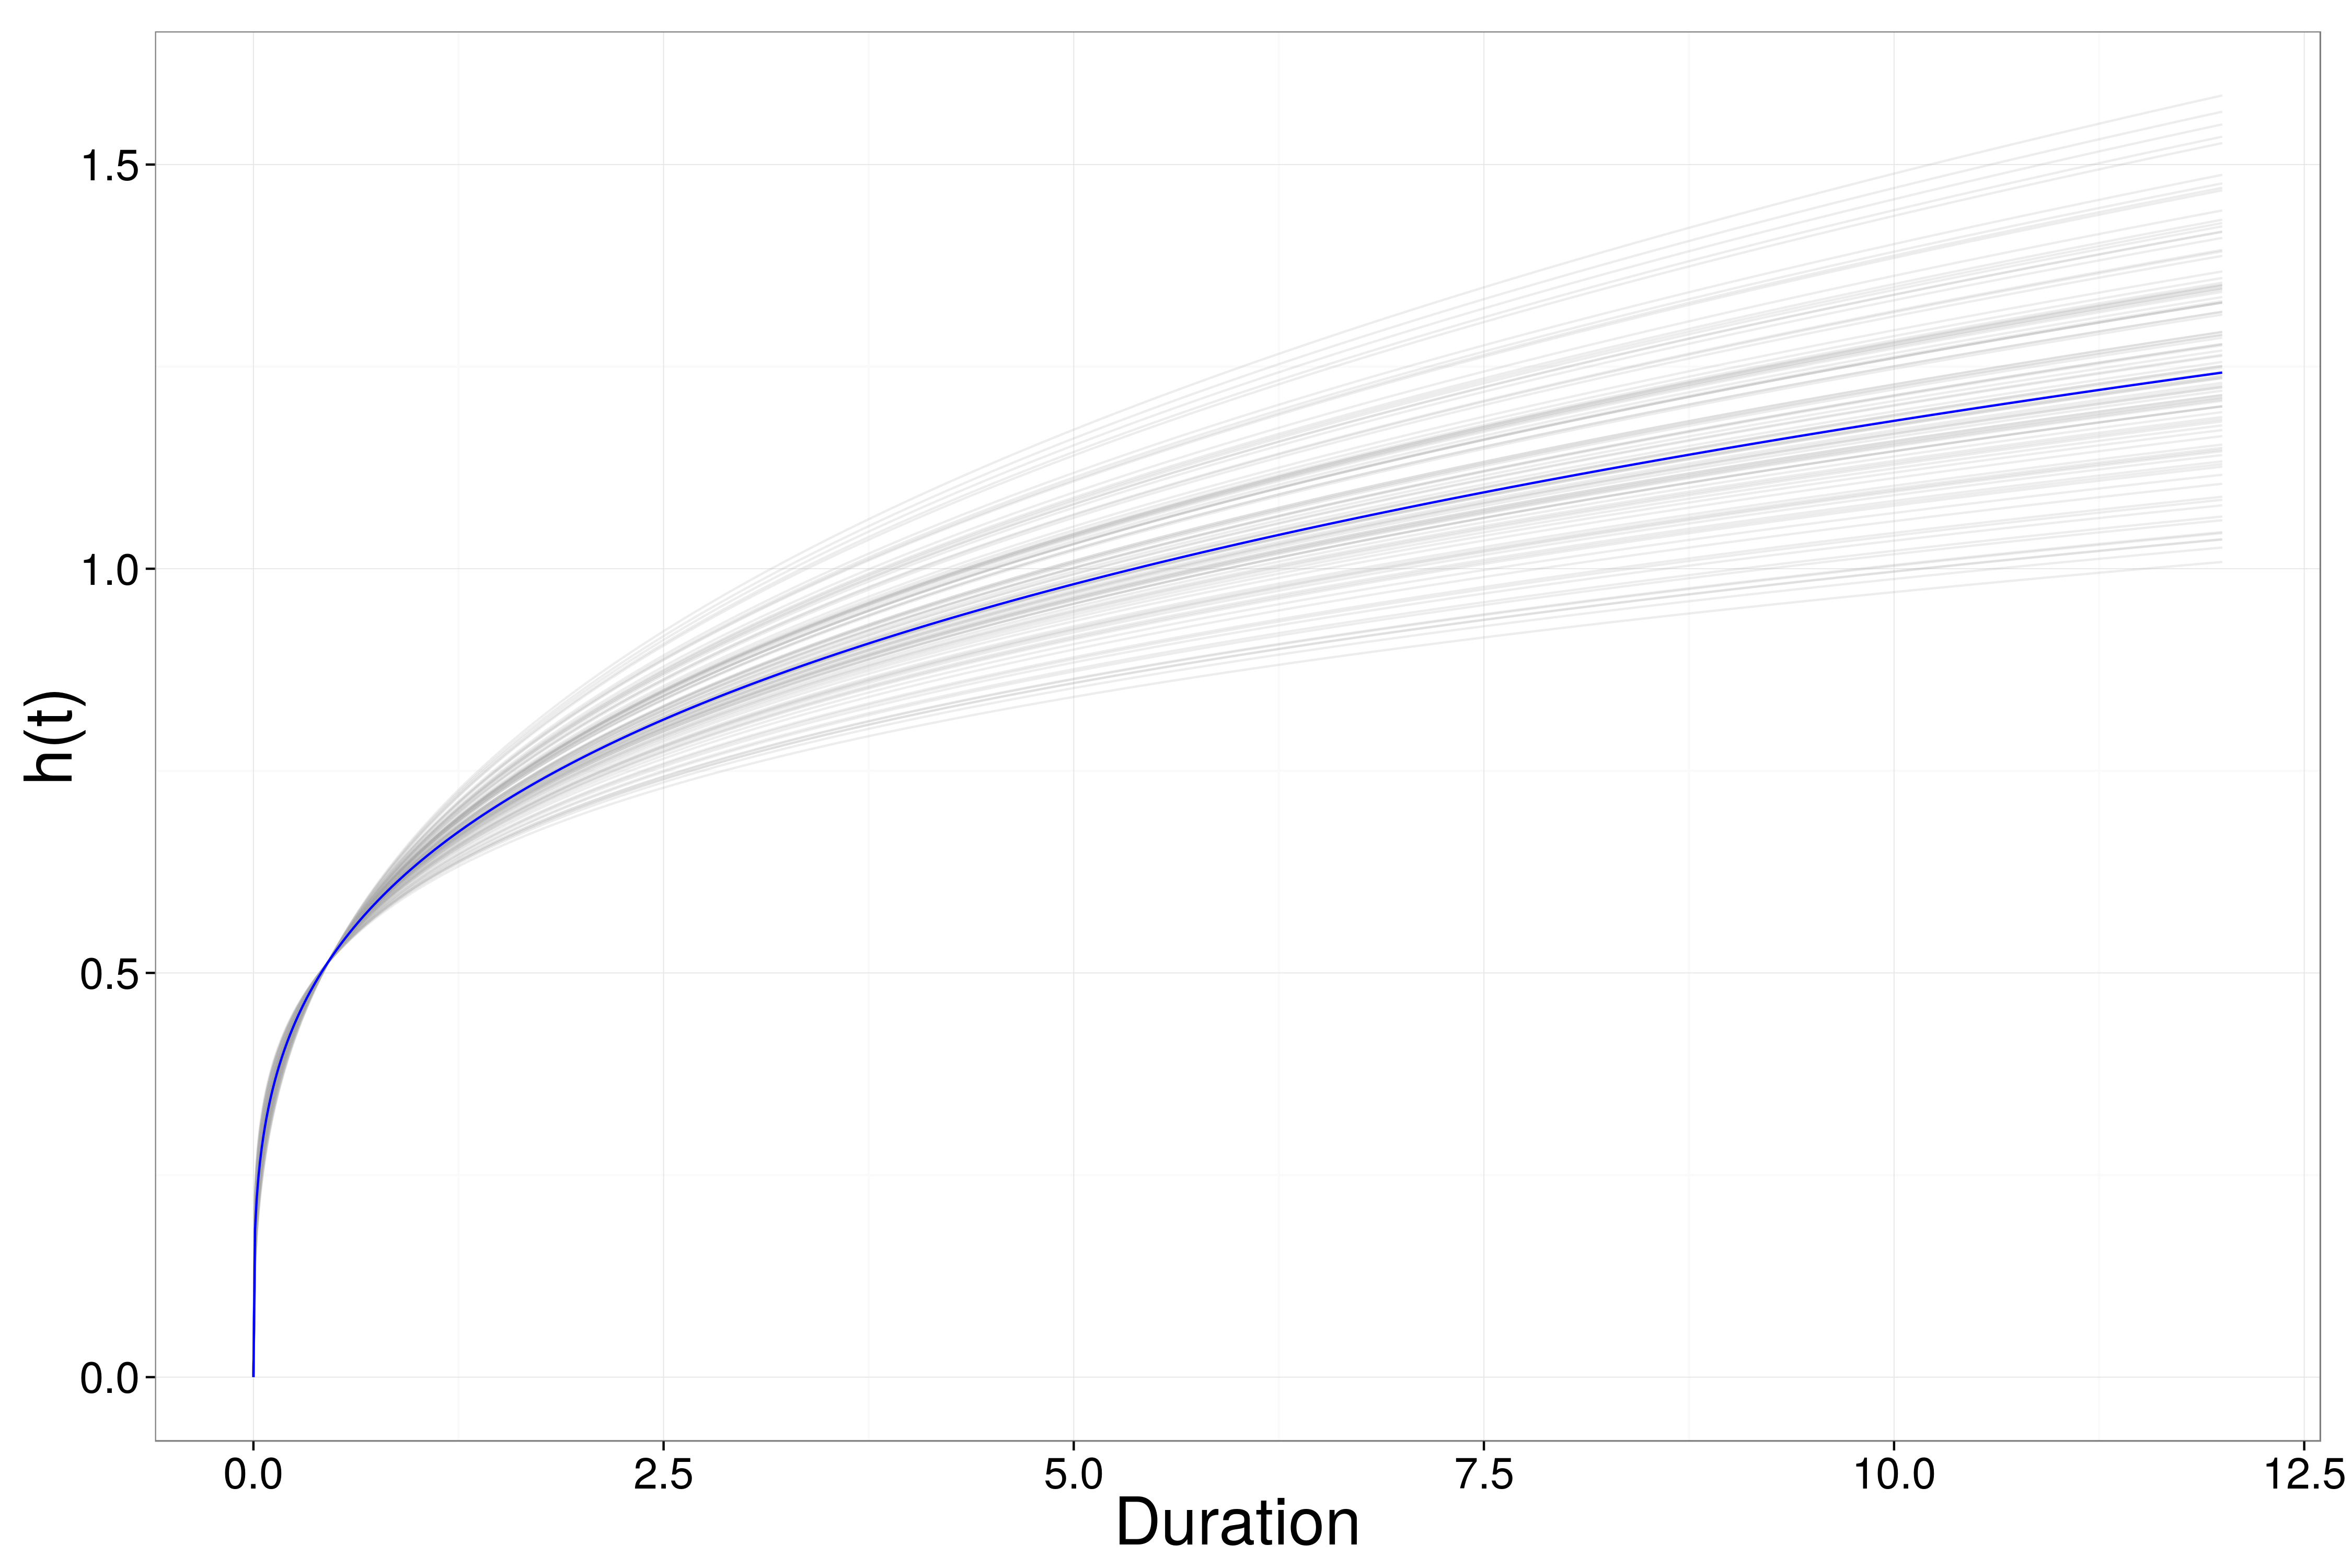
\includegraphics[height = 0.8\textheight, width = \textwidth,  keepaspectratio = true]{figure/haz_est}
  \end{center}
\end{frame}

\begin{frame}
  \frametitle{Meaning}
  \begin{columns}
    \begin{column}{0.5\textwidth}
      Results
      \begin{itemize}
        \item comparable probabilistic statements of trait, temporal, and historical effects
        \item increasing cohort survival risk over Cenozoic
        \item \(h(t)\) not constant over \(t\), increases
        \item model fits; no systematic biases in residuals, though noisy.
      \end{itemize}
    \end{column}
    \begin{column}{0.5\textwidth}
      Interpretation
      \begin{itemize}
        \item older lineages out-competed by younger (Wagner and Estabrook '14 \textit{PNAS})
        \item increasing extinction with group age (Quental and Marshall '13 \textit{Science})
        \item background extinction and the blurring of Raup's modes of extinction
        \item relative effect of each covariate, levels of selection(?)
      \end{itemize}
    \end{column}
  \end{columns}
\end{frame}


\begin{frame}
  A model of biological, spatial, and phylogenic effects on Cenozoic mammal co-occurrence
\end{frame}

\begin{frame}
  \frametitle{Biogeographic network}
\end{frame}

\begin{frame}
  \frametitle{Species adjacency}
\end{frame}

\begin{frame}
  \frametitle{Random graphs}

  Erdos-Renyi graph \(G(n, p)\)

  Poisson distributed degree
\end{frame}

\begin{frame}
  \frametitle{Model diagram}
  \begin{center}
    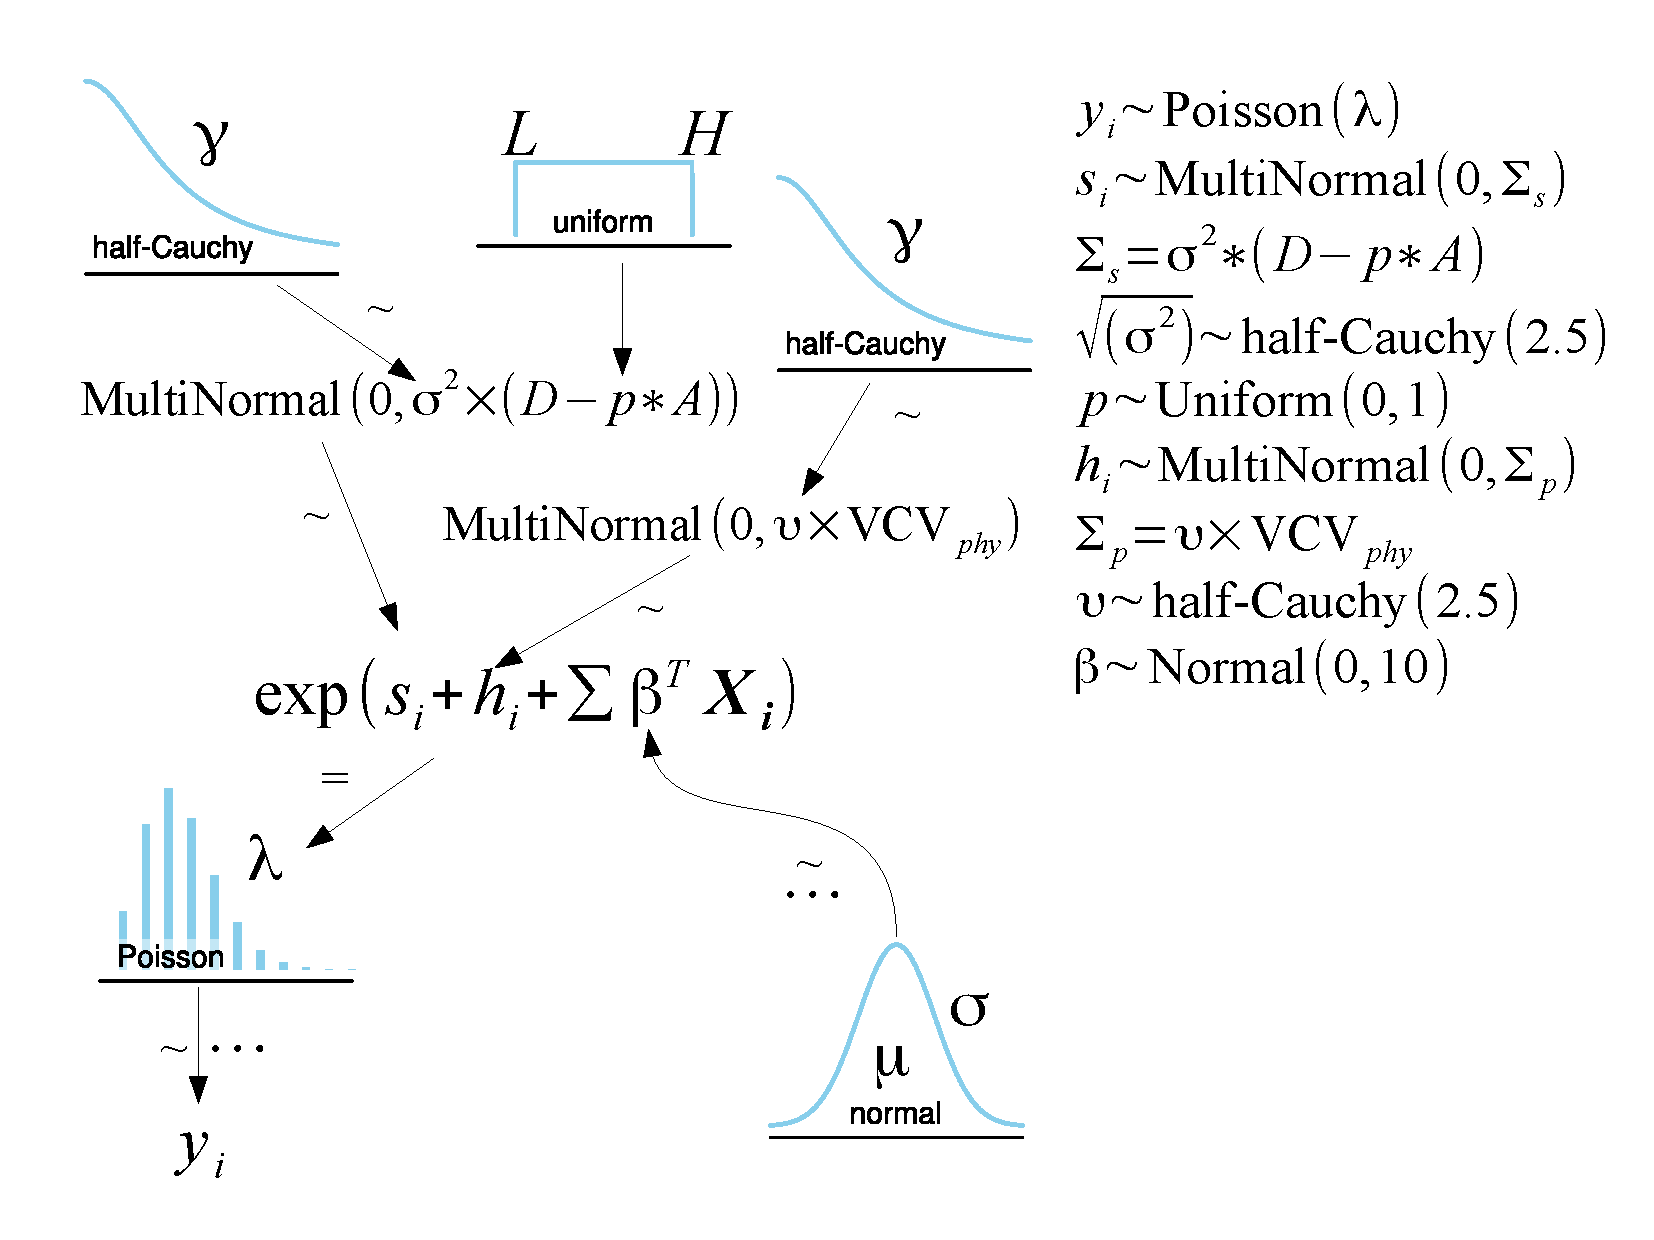
\includegraphics[height = 0.8\textheight, width = \textwidth,  keepaspectratio = true]{figure/mammal_degree_model}
  \end{center}
\end{frame}

% Do I want to try and show some results?


\end{document}
